% Options for packages loaded elsewhere
\PassOptionsToPackage{unicode}{hyperref}
\PassOptionsToPackage{hyphens}{url}
%
\documentclass[
  a4paper,
]{book}
\usepackage{amsmath,amssymb}
\usepackage{iftex}
\ifPDFTeX
  \usepackage[T1]{fontenc}
  \usepackage[utf8]{inputenc}
  \usepackage{textcomp} % provide euro and other symbols
\else % if luatex or xetex
  \usepackage{unicode-math} % this also loads fontspec
  \defaultfontfeatures{Scale=MatchLowercase}
  \defaultfontfeatures[\rmfamily]{Ligatures=TeX,Scale=1}
\fi
\usepackage{lmodern}
\ifPDFTeX\else
  % xetex/luatex font selection
\fi
% Use upquote if available, for straight quotes in verbatim environments
\IfFileExists{upquote.sty}{\usepackage{upquote}}{}
\IfFileExists{microtype.sty}{% use microtype if available
  \usepackage[]{microtype}
  \UseMicrotypeSet[protrusion]{basicmath} % disable protrusion for tt fonts
}{}
\makeatletter
\@ifundefined{KOMAClassName}{% if non-KOMA class
  \IfFileExists{parskip.sty}{%
    \usepackage{parskip}
  }{% else
    \setlength{\parindent}{0pt}
    \setlength{\parskip}{6pt plus 2pt minus 1pt}}
}{% if KOMA class
  \KOMAoptions{parskip=half}}
\makeatother
\usepackage{xcolor}
\usepackage{color}
\usepackage{fancyvrb}
\newcommand{\VerbBar}{|}
\newcommand{\VERB}{\Verb[commandchars=\\\{\}]}
\DefineVerbatimEnvironment{Highlighting}{Verbatim}{commandchars=\\\{\}}
% Add ',fontsize=\small' for more characters per line
\usepackage{framed}
\definecolor{shadecolor}{RGB}{248,248,248}
\newenvironment{Shaded}{\begin{snugshade}}{\end{snugshade}}
\newcommand{\AlertTok}[1]{\textcolor[rgb]{0.94,0.16,0.16}{#1}}
\newcommand{\AnnotationTok}[1]{\textcolor[rgb]{0.56,0.35,0.01}{\textbf{\textit{#1}}}}
\newcommand{\AttributeTok}[1]{\textcolor[rgb]{0.13,0.29,0.53}{#1}}
\newcommand{\BaseNTok}[1]{\textcolor[rgb]{0.00,0.00,0.81}{#1}}
\newcommand{\BuiltInTok}[1]{#1}
\newcommand{\CharTok}[1]{\textcolor[rgb]{0.31,0.60,0.02}{#1}}
\newcommand{\CommentTok}[1]{\textcolor[rgb]{0.56,0.35,0.01}{\textit{#1}}}
\newcommand{\CommentVarTok}[1]{\textcolor[rgb]{0.56,0.35,0.01}{\textbf{\textit{#1}}}}
\newcommand{\ConstantTok}[1]{\textcolor[rgb]{0.56,0.35,0.01}{#1}}
\newcommand{\ControlFlowTok}[1]{\textcolor[rgb]{0.13,0.29,0.53}{\textbf{#1}}}
\newcommand{\DataTypeTok}[1]{\textcolor[rgb]{0.13,0.29,0.53}{#1}}
\newcommand{\DecValTok}[1]{\textcolor[rgb]{0.00,0.00,0.81}{#1}}
\newcommand{\DocumentationTok}[1]{\textcolor[rgb]{0.56,0.35,0.01}{\textbf{\textit{#1}}}}
\newcommand{\ErrorTok}[1]{\textcolor[rgb]{0.64,0.00,0.00}{\textbf{#1}}}
\newcommand{\ExtensionTok}[1]{#1}
\newcommand{\FloatTok}[1]{\textcolor[rgb]{0.00,0.00,0.81}{#1}}
\newcommand{\FunctionTok}[1]{\textcolor[rgb]{0.13,0.29,0.53}{\textbf{#1}}}
\newcommand{\ImportTok}[1]{#1}
\newcommand{\InformationTok}[1]{\textcolor[rgb]{0.56,0.35,0.01}{\textbf{\textit{#1}}}}
\newcommand{\KeywordTok}[1]{\textcolor[rgb]{0.13,0.29,0.53}{\textbf{#1}}}
\newcommand{\NormalTok}[1]{#1}
\newcommand{\OperatorTok}[1]{\textcolor[rgb]{0.81,0.36,0.00}{\textbf{#1}}}
\newcommand{\OtherTok}[1]{\textcolor[rgb]{0.56,0.35,0.01}{#1}}
\newcommand{\PreprocessorTok}[1]{\textcolor[rgb]{0.56,0.35,0.01}{\textit{#1}}}
\newcommand{\RegionMarkerTok}[1]{#1}
\newcommand{\SpecialCharTok}[1]{\textcolor[rgb]{0.81,0.36,0.00}{\textbf{#1}}}
\newcommand{\SpecialStringTok}[1]{\textcolor[rgb]{0.31,0.60,0.02}{#1}}
\newcommand{\StringTok}[1]{\textcolor[rgb]{0.31,0.60,0.02}{#1}}
\newcommand{\VariableTok}[1]{\textcolor[rgb]{0.00,0.00,0.00}{#1}}
\newcommand{\VerbatimStringTok}[1]{\textcolor[rgb]{0.31,0.60,0.02}{#1}}
\newcommand{\WarningTok}[1]{\textcolor[rgb]{0.56,0.35,0.01}{\textbf{\textit{#1}}}}
\usepackage{longtable,booktabs,array}
\usepackage{calc} % for calculating minipage widths
% Correct order of tables after \paragraph or \subparagraph
\usepackage{etoolbox}
\makeatletter
\patchcmd\longtable{\par}{\if@noskipsec\mbox{}\fi\par}{}{}
\makeatother
% Allow footnotes in longtable head/foot
\IfFileExists{footnotehyper.sty}{\usepackage{footnotehyper}}{\usepackage{footnote}}
\makesavenoteenv{longtable}
\usepackage{graphicx}
\makeatletter
\def\maxwidth{\ifdim\Gin@nat@width>\linewidth\linewidth\else\Gin@nat@width\fi}
\def\maxheight{\ifdim\Gin@nat@height>\textheight\textheight\else\Gin@nat@height\fi}
\makeatother
% Scale images if necessary, so that they will not overflow the page
% margins by default, and it is still possible to overwrite the defaults
% using explicit options in \includegraphics[width, height, ...]{}
\setkeys{Gin}{width=\maxwidth,height=\maxheight,keepaspectratio}
% Set default figure placement to htbp
\makeatletter
\def\fps@figure{htbp}
\makeatother
\setlength{\emergencystretch}{3em} % prevent overfull lines
\providecommand{\tightlist}{%
  \setlength{\itemsep}{0pt}\setlength{\parskip}{0pt}}
\setcounter{secnumdepth}{5}
\usepackage{booktabs}

\usepackage{titlesec, environ}
\newif\ifcomm\commtrue
\NewEnviron{myanswers}{\ifcomm\BODY\fi}
\ifLuaTeX
  \usepackage{selnolig}  % disable illegal ligatures
\fi
\usepackage[]{natbib}
\bibliographystyle{plainnat}
\usepackage{bookmark}
\IfFileExists{xurl.sty}{\usepackage{xurl}}{} % add URL line breaks if available
\urlstyle{same}
\hypersetup{
  pdftitle={MATH1710 Probability and Statistics I},
  pdfauthor={Matthew Aldridge},
  hidelinks,
  pdfcreator={LaTeX via pandoc}}

\title{MATH1710 Probability and Statistics I}
\author{\href{https://mpaldridge.github.io/}{Matthew Aldridge}}
\date{University of Leeds, 2023--24}

\usepackage{amsthm}
\newtheorem{theorem}{Theorem}[chapter]
\newtheorem{lemma}{Lemma}[chapter]
\newtheorem{corollary}{Corollary}[chapter]
\newtheorem{proposition}{Proposition}[chapter]
\newtheorem{conjecture}{Conjecture}[chapter]
\theoremstyle{definition}
\newtheorem{definition}{Definition}[chapter]
\theoremstyle{definition}
\newtheorem{example}{Example}[chapter]
\theoremstyle{definition}
\newtheorem{exercise}{Exercise}[chapter]
\theoremstyle{definition}
\newtheorem{hypothesis}{Hypothesis}[chapter]
\theoremstyle{remark}
\newtheorem*{remark}{Remark}
\newtheorem*{solution}{Solution}
\begin{document}
\maketitle

{
\setcounter{tocdepth}{1}
\tableofcontents
}
\chapter*{Schedule}\label{schedule}
\addcontentsline{toc}{chapter}{Schedule}

\newcommand{\Var}{\operatorname{Var}}

\textbf{Week 10} (4--8 December):

\begin{itemize}
\tightlist
\item
  \hyperref[L19-bayes-i]{\textbf{Lecture 19:} Bayesian statistics I} (Monday 4 December)
\item
  \hyperref[L20-bayes-ii]{\textbf{Lecture 20:} Bayesian statistics II} (Wednesday 8 December)
\item
  \textbf{Tutorial} on Problem Sheet 5
\item
  \hyperref[P5]{\textbf{Problem Sheet 5:}} Work through in preparation for your tutorial. Deadline for assessed questions: Monday 11 December.
\item
  \hyperref[R]{\textbf{R Worksheet 9}} -- no assessed questions
\item
  \hyperref[R]{\textbf{R Worksheet 10}} is available early -- deadline for assessed questions: Thursday 14 December
\item
  \textbf{Office hours:} Friday 1 December, 11--12 and 1--2, \href{https://mpaldridge.github.io/office.html}{Physics Research Deck 9.320}
\end{itemize}

\textbf{Week 9} (27 November -- 1 December):

\begin{itemize}
\tightlist
\item
  \hyperref[L17-exponential-multi]{\textbf{Lecture 17:} Exponential distribution and multiple continuous random variables} (Monday 27 November)
\item
  \hyperref[L18-limit]{\textbf{Lecture 18:} Limit theorems} (Wednesday 29 November)
\item
  \hyperref[P5]{\textbf{Problem Sheet 5:}} Work through in preparation for your tutorial in Week 10. Deadline for assessed questions: Monday 11 December.
\item
  \hyperref[R]{\textbf{R Worksheet 8}} -- deadline for assessed questions: Monday 4 December
\item
  \textbf{Office hours:} Friday 1 December, 11--12 and 1--2, \href{https://mpaldridge.github.io/office.html}{Physics Research Deck 9.320}
\end{itemize}

\textbf{Week 8} (20--24 November):

\begin{itemize}
\tightlist
\item
  \hyperref[L15-continuous]{\textbf{Lecture 15:} Continuous random variables} (Monday 20 November)
\item
  \hyperref[L16-normal]{\textbf{Lecture 16:} Normal distribution} (Wednesday 22 November)
\item
  \textbf{Tutorial} on \hyperref[P4]{Problem Sheet 4}
\item
  \hyperref[P4]{\textbf{Problem Sheet 4:}} Work through in preparation for your tutorial. Deadline for assessed questions: Monday 27 November.
\item
  \hyperref[R]{\textbf{R Worksheet 7}}
\item
  \textbf{Office hours:} Friday 24 November, 11--12 and 1--2, \href{https://mpaldridge.github.io/office.html}{Physics Research Deck 9.320}
\end{itemize}

\textbf{Week 7} (13--17 November):

\begin{itemize}
\tightlist
\item
  \hyperref[L13-multi-rv]{\textbf{Lecture 13:} Multiple random variables} (Monday 13 November)
\item
  \hyperref[L14-covariance]{\textbf{Lecture 14:} Expectation and covariance} (Wednesday 15 November)
\item
  \hyperref[P4]{\textbf{Problem Sheet 4:}} Work through in preparation for your tutorial in Week 8. Deadline for assessed questions: Monday 27 November.
\item
  \hyperref[R]{\textbf{R Worksheet 6:}} -- deadline for assessed questions: Monday 20 November
\item
  \textbf{Office hours:} Friday 17 November, 11--12 and 1--2, \href{https://mpaldridge.github.io/office.html}{Physics Research Deck 9.320}
\end{itemize}

\textbf{Week 6} (6--10 November):

\begin{itemize}
\tightlist
\item
  \hyperref[L11-binomial-geometric]{\textbf{Lecture 11:} Binomial and geometric distributions} (Monday 6 November)
\item
  \hyperref[L12-poisson]{\textbf{Lecture 12:} Poisson distribution} (Wednesday 8 November)
\item
  \textbf{Tutorial} on Problem Sheet 3
\item
  \hyperref[P3]{\textbf{Problem Sheet 3:}} Work through in preparation for your tutorial. Deadline for assessed questions: Monday 13 November.
\item
  \hyperref[R]{\textbf{R Worksheet 5}}
\item
  \textbf{Office hours:} Friday 10 November, 11--12 and 1--2, \href{https://mpaldridge.github.io/office.html}{Physics Research Deck 9.320}
\item
  \href{https://forms.office.com/e/8ETiji58Zi}{Mid-semester check-in}
\end{itemize}

\textbf{Week 5} (30 October--3 November):

\begin{itemize}
\tightlist
\item
  \hyperref[L09-discrete-rv]{\textbf{Lecture 9:} Discrete random variables} (Monday 30 October)
\item
  \hyperref[L10-expectation]{\textbf{Lecture 10:} Expectation and variance} (Wednesday 1 November)
\item
  \hyperref[P3]{\textbf{Problem Sheet 3:}} Work through in preparation for your tutorial in Week 6. Deadline for assessed questions: Monday 13 November.
\item
  \hyperref[R]{\textbf{R Worksheet 4}} -- deadline for assessed questions: Monday 6 November
\item
  \textbf{Office hours:} Friday 3 November, 11--1, \href{https://mpaldridge.github.io/office.html}{Physics Research Deck 9.320} (\emph{note change of time})
\end{itemize}

\textbf{Week 4} (23--27 October):

\begin{itemize}
\tightlist
\item
  \hyperref[L07-conditional]{\textbf{Lecture 7:} Independence and conditional probabilty} (Monday 23 October)
\item
  \hyperref[L08-two-theorems]{\textbf{Lecture 8:} Two theorems on conditional probability} (Wednesday 25 October)
\item
  \textbf{Tutorial} on \hyperref[P2]{Problem Sheet 2}
\item
  \hyperref[P2]{\textbf{Problem Sheet 2:}} Work through in preparation for your tutorial. Deadline for assessed questions: Monday 30 October.
\item
  \hyperref[R]{\textbf{R Worksheet 3}}
\item
  \textbf{Office hours:} Friday 27 October, 11--12 and 1--2, \href{https://mpaldridge.github.io/office.html}{Physics Research Deck 9.320} (\emph{note change of venue})
\end{itemize}

\textbf{Week 3} (16--20 October):

\begin{itemize}
\tightlist
\item
  \hyperref[L05-classical-i]{\textbf{Lecture 5:} Classical probability I} (Monday 16 October)
\item
  \hyperref[L06-classical-ii]{\textbf{Lecture 6:} Classical probability II} (Wednesday 18 October)
\item
  \textbf{R Practical}
\item
  \hyperref[P2]{\textbf{Problem Sheet 2:}} Work through in preparation for your tutorial in Week 4. Deadline for assessed questions: Monday 30 October.
\item
  \hyperref[R]{\textbf{R Worksheet 2:}} Deadline for assessed exercises: Monday 23 October
\item
  \textbf{Office hours:} Friday 20 October, 11--12 and 1--2, \href{boardroom.png}{Maths Boardroom}
\end{itemize}

\textbf{Week 2} (9--13 October):

\begin{itemize}
\tightlist
\item
  \hyperref[L03-events]{\textbf{Lecture 3:} Sample spaces and events} (Monday 9 October)
\item
  \hyperref[L04-probability]{\textbf{Lecture 4:} Probability} (Wednesday 11 October)
\item
  \textbf{Tutorial} on \hyperref[P1]{Problem Sheet 1}
\item
  \hyperref[practical]{\textbf{R Practical}}
\item
  \hyperref[P1]{\textbf{Problem Sheet 1:}} Work through in preparation for your tutorial. Deadline for assessed questions: Monday 16 October.
\item
  \hyperref[R]{\textbf{R Worksheet 1}}
\item
  \textbf{Office hours:} Friday 13 October, 11--12 and 1--2, \href{boardroom.png}{Maths Boardroom}
\end{itemize}

\textbf{Week 1} (2--6 October):

\begin{itemize}
\tightlist
\item
  \hyperref[L01-stats]{\textbf{Lecture 1:} Summary statistics} (Monday 2 October)
\item
  \hyperref[L02-dataviz]{\textbf{Lecture 2:} Data visualisation} (Wednesday 4 October)
\item
  \hyperref[P1]{\textbf{Problem Sheet 1:}} Work through in preparation for your tutorial in Week 2. Deadline for assessed questions: Monday 16 October.
\item
  \textbf{Office hours:} Friday 6 October, 11--12 and 1--2, \href{boardroom.png}{Maths Boardroom}
\end{itemize}

\part*{Part II: Probability}\label{part-part-ii-probability}
\addcontentsline{toc}{part}{Part II: Probability}

\chapter{Sample spaces and events}\label{L03-events}

\renewcommand{\complement}{\mathsf{c}}
\newcommand{\comp}{\complement}
\newcommand{\ff}[2]{{#1}^{\underline{#2}}}

\section{What is probability?}\label{what-is-prob}

We now begin the big central block of this module, on probability theory.

Probability theory is the study of randomness. Probability, as an area of mathematics, is a fascinating subject in its own right. However, probability is particularly important due to its usefulness in applications -- especially in statistics (the study of data), in finance, and in actuarial science (the study of insurance).

Probability is well suited to modelling situations that involve randomness, uncertainty, or unpredictability. If you want to predict the time of the next solar eclipse, a deterministic (that is, non-random) model based on physical laws will tell you when the sun, the moon, and the earth will be in the correct positions; but if you want to predict the weather tomorrow, or the price of a share of Apple stock next month, or the results of an election next year, you will need a probabilistic model that takes into account the uncertainty in the outcome. A probabilistic model could tell you the most likely outcome, or a range of the most probable outcomes.

So what do we mean when we talk about the ``probability'' of an event occurring? You might say that the probability of an event is a measure of ``how likely'' it is to occur, or what the ``chance'' of it occurring is.

More concretely, here are some interpretations of probability:

\begin{itemize}
\tightlist
\item
  \textbf{Subjective} (or \textbf{Bayesian}) \textbf{probability:} The probability of an event is the way someone expresses their degree of belief that the event will occur, based on their own judgement, and given the evidence they have seen. Their belief is measured on a scale from 0 to 1, from probabilities near 0 meaning they believe the event is very unlikely to occur to probabilities near 1 meaning they believe the event is very likely to occur.

  \begin{itemize}
  \tightlist
  \item
    This interpretation is philosophically sound, but a bit vague to be the basis for a mathematics module.
  \end{itemize}
\item
  \textbf{Classical} (or \textbf{enumerative}) \textbf{probability:} Suppose there are a finite number of equally likely outcomes. Then the probability of an event is the proportion of those outcomes that correspond to the event occurring. So when we say that a randomly dealt card has a probability \(\frac{1}{13}\) of being an ace, this is because there are 52 cards of which 4 are aces, so the proportion of favourable outcomes is \(\frac{4}{52} = \frac{1}{13}\).

  \begin{itemize}
  \tightlist
  \item
    This interpretation is good for simple procedures like flipping a fair coin, rolling a dice, or dealing cards, where the ``finite number of equally likely outcomes'' assumption holds. But we want to be able to study more complicated situations, where some outcomes are more likely than others, or where infinitely many different outcomes are possible.
  \end{itemize}
\item
  \textbf{Frequentist probability:} In a repeated experiment, the probability of an event is its long-run frequency. That is, if we repeat an experiment a very large number of times, the probability of the event is (approximately) the proportion of the experiments in which the event occurs. So when we say a biased coin has probability 0.9 of landing heads, we mean that were we toss it 1000 times, we would expect to see very close to \(0.9 \times 1000 = 900\) heads.

  \begin{itemize}
  \tightlist
  \item
    There are two problems with this. First, this doesn't deal with events that can't be repeated over and over again (like ``What's the probability that Labour win the 2024 general election?''). Second, to answer the question, ``Yes, but \emph{how} close to the probability should the proportion of occurrences be?'', you end up having to answer, ``Well, it depends on the probability,'' and you've got a circular definition.
  \end{itemize}
\item
  \textbf{Mathematical probability:} We have a function that assigns to each event a number between 0 and 1, called its probability, and that function has to obey certain mathematical rules, called ``axioms''.
\end{itemize}

It will not surprise you to learn that, in this mathematics course, we will take the ``mathematical probability'' approach. However, we will also learn useful things about the other approaches: we will see that classical probability is one special case of mathematical probability; we will see a result called the ``law of large numbers'' that says that the long-run frequency does indeed get closer and closer to the mathematical probability; and a result called ``Bayes' theorem'' will advise a subjectivist on how to update her subjective beliefs when she sees new evidence.

\section{Sample spaces and events}\label{sample-events}

Taking the ``mathematical probability'' approach, we will want to give a formal mathematical definition of the \emph{probability} of an event. But even before that, we need to give a formal mathematical definition of an \emph{event} itself. Our setup will be this:

\begin{itemize}
\tightlist
\item
  There is a set called the \textbf{sample space}, normally given the letter \(\Omega\) (upper-case Omega), which is the set of all possible outcomes.
\item
  An element of the sample space \(\Omega\) is a \textbf{sample outcome}, sometimes given the letter \(\omega\) (lower-case omega), represents one of the possible outcomes.
\item
  An \textbf{event} is a set of sample outcomes; that is, a subset of the sample space \(\Omega\). Events are often given letters like \(A\), \(B\), \(C\). We write \(A \subset \Omega\) to mean that \(A\) is an event in (or, equivalently, is a subset of) the sample space \(\Omega\).
\end{itemize}

This will be easier to understand with some concrete examples. We write a set (such as a sample space or an event) by writing all the elements of that set inside curly brackets \(\{\ \}\), separated by commas.

\begin{example}
Suppose we toss a (possibly biased) coin, and record whether it lands heads or tails. Then our sample space is \(\Omega = \{\mathrm H, \mathrm T\}\), where the sample outcome H denotes heads and the sample outcome T denotes tails.

The event that the coin lands heads is \(\{\mathrm H\}\).
\end{example}

\begin{example}
Suppose we roll a dice, and record the number rolled. Then our sample space is \(\Omega = \{1,2,3,4,5,6\}\), where the sample outcome \(1\) corresponds to rolling a one, and so on.

The event ``we roll an even number'' is \(\{2,4,6\}\). The event ``we roll at least a five'' is \(\{5,6\}\).
\end{example}

\begin{example}
Suppose we wish to count how many claims are made to an insurance company in a year. We could model this by taking the sample space \(\Omega\) to be \(\mathbb Z_+ = \{0, 1, 2, \dots\}\), the set of all non-negative integers.

The event ``the company receives less than 1000 claims'' is \(\{0, 1, 2, \dots, 998, 999\}\).
\end{example}

\begin{example}
Suppose we want a computer to pick a random number between 0 and 1. We could model this by taking the sample space \(\Omega\) to be the interval \([0, 1]\) of all real numbers between 0 and 1.

The event ``the number is bigger than \(\frac12\)'' is the sub-interval \((\frac12, 1]\) of all real numbers greater than \(\frac12\) but no bigger than 1. The event ``the first digit is a 7'' is the sub-interval \([0.7, 0.8)\). The event ``the random number is exactly \(1/\sqrt{2}\)'' is \(\{1/\sqrt{2}\}\).
\end{example}

In the first two examples, the sample space \(\Omega\) was finite. In third example, the sample space was infinite but ``countably infinite'', in that it could be counted using the discrete values of the positive integers. Both of these were for \emph{counting} discrete observations. In the fourth example, the sample space was infinite but ``uncountably infinite'', in that it had a sliding scale or ``continuum'' of gradually varying measurements. This was for \emph{measuring} continuous observations. This distinction will be important later in the course.

For any sample space \(\Omega\), there are two special events that always exist. There's \(\Omega\) itself, the event containing all of the sample outcomes, which represents ``something happens''. There's also the empty set \(\varnothing\), which contains none of the sample outcomes, which represents ``nothing happens''. Common sense suggests that \(\Omega\) should have probability 1, because \emph{something} is bound to happen -- this will later be one of our probability ``axioms''. Common sense also suggests that \(\varnothing\) should have probability 0, because it can't be that \emph{nothing} happens -- this will not be one probability axioms, but we'll show that it follows logically from the axioms we do choose.

\section{Set theory}\label{set-theory}

Since we've now defined events as being sets -- specifically, subsets of the sample space \(\Omega\) -- it will be useful to mention a little set basic theory here.

First, there are ways we can build new sets (or events) out of old. It's fine to just read the words and look at the pictures for these definitions, but those who want to read the equations too will need to know this:

\begin{itemize}
\tightlist
\item
  \(\omega \in A\) means ``\(\omega\) is in \(A\)'' or ``\(\omega\) is an element of \(A\)'', while \(\omega \not\in A\) means the opposite, that \(\omega\) is \emph{not} in \(A\);
\item
  a colon \(:\) in the middle of set notation should be read as ``such that'';
\item
  so \(\{\omega \in \Omega : \text{fact about $\omega$}\}\) should be read as ``the set of sample outcomes \(\omega\) in the sample space \(\Omega\) such that the fact is true''.
\end{itemize}

\begin{definition}

Consider a sample space \(\Omega\), and let \(A\) and \(B\) be events in that sample space.

\begin{itemize}
\tightlist
\item
  \textbf{{NOT:}} The \textbf{complement} of \(A\), written \(A^\mathsf{c}\) (and said ``\(A\) complement'' or ``not \(A\)''), is the set of sample outcomes not in \(A\); that is
  \[ A^\mathsf{c}= \{\omega \in \Omega : \omega \not\in A \} . \]
  This represents the event that \(A\) does not occur.
\item
  \textbf{{AND}:} The \textbf{intersection} of \(A\) and \(B\), written \(A \cap B\) (and said ``\(A\) intersect \(B\)'' or ``\(A\) and \(B\)'') is the set of sample outcomess in both \(A\) and \(B\); that is,\\
  \[ A \cap B = \{\omega \in \Omega : \omega \in A \text{ and } \omega \in B \} . \]
  This represents the event that both \(A\) and \(B\) occur.
\item
  \textbf{{OR:}} The \textbf{union} of \(A\) and \(B\), written \(A \cup B\) (and said ``\(A\) union \(B\)'' or ``\(A\) or \(B\)'') is the set of sample outcomess in \(A\) or in \(B\); that is,
  \[ A \cup B = \{\omega \in \Omega : \omega \in A \text{ or } \omega \in B \} . \]
  This represents the event that \(A\) occurs or \(B\) occurs. (In mathematics, ``or'' includes ``both'', so a sample outcome in both \(A\) and \(B\) is in \(A\cup B\) too.)
\end{itemize}

~

\begin{center}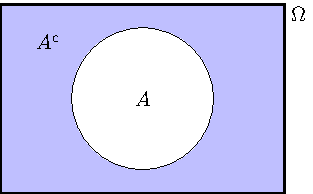
\includegraphics[width=550pt]{math1710_files/figure-latex/venn-not-1} \end{center}

\begin{center}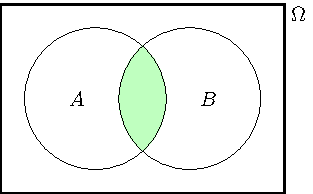
\includegraphics[width=550pt]{math1710_files/figure-latex/venn-and-1} \end{center}

\begin{center}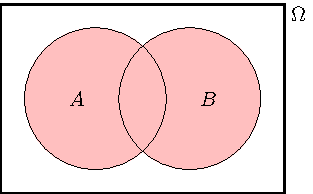
\includegraphics[width=550pt]{math1710_files/figure-latex/venn-or-1} \end{center}

\end{definition}

\begin{example}
Suppose we are rolling a dice, so our sample space is \(\Omega = \{1,2,3,4,5,6\}\). Let \(A = \{2,4,6\}\) be the event that we roll and even number, and let \(B = \{5,6\}\) be the event that we roll at least a 5. Then
\begin{align*}
A^\mathsf{c}&= \{1,3,5\} = \{\text{roll an odd number}\} ,\\
A \cap B &= \{6\} = \{\text{roll a 6}\} ,\\
A \cup B &= \{2,4,5,6\} .
\end{align*}
\end{example}

An important case is when two events \(A, B\) cannot happen at the same time; that is, \(A \cap B = \varnothing\) (``\(A\) intersect \(B\) is the empty set''). In this case, we say that \(A\) and \(B\) are \textbf{disjoint} or \textbf{mutually exclusive}. For example, when \(\Omega\) is \href{https://en.wikipedia.org/wiki/Standard_52-card_deck}{a deck of cards}, then \(A = \{\text{the card is a spade}\}\) and \(B = \{\text{the card is red}\}\) are disjoint, because a card cannot be both a spade (a black suit) and red.

You might think that if two events are disjoint, then it would be reasonable to find the probability of their union -- that is, the probability that one (and, by necessity, only one) of them happens -- you can just add the two separate probabilities together. This will be another of our ``axioms'' of probability.

There are a few rules about ways you can combine the complement, intersection and union operations. These are ways of building new events from old.

\begin{itemize}
\tightlist
\item
  The \textbf{double complement law} tells us that not-not-\(A\) is the same as \(A\):
  \[ (A^\mathsf{c})^\mathsf{c}= A .\]
  This says that if it's not ``not-raining'', then it's raining!
\item
  The \textbf{distributive laws} tells us we can ``multiply out of the brackets'' with sets:
  \begin{align*}
  A \cap (B \cup C) &= (A \cap B) \cup (A \cap C) ,\\
  A \cup (B \cap C) &= (A \cup B) \cap (A \cup C) .
  \end{align*}
  The first says that if you are eating a burger with fries or salad, then you're eating a burger with fries or eating a burger with salad. The second is a bit less intuitive, I find, but it's clear that if \(A\) is true then the first of each of the terms on the right is true, while if both \(B\) and \(C\) are true then the second of each of the terms on the right is true.
\item
  \textbf{De Morgan's laws} tell us how complements interact with intersection/unions:
  \begin{align*}
  (A \cap B)^\mathsf{c}&= A^\mathsf{c}\cup B^\mathsf{c}\\
  (A \cup B)^\mathsf{c}&= A^\mathsf{c}\cap B^\mathsf{c}
  \end{align*}
  The first of these says that if it's not a Monday in October, then either it's not Monday or it's not October (or both). The second says that if a maths lecture is not ``useful or fun'', then it's not useful and it's not fun. (\href{https://mathshistory.st-andrews.ac.uk/Biographies/De_Morgan/}{Augustus De Morgan} was a British mathematician of the 19th century who did important work in logic.)
\end{itemize}

For this module, these mostly count as ``common sense'' -- but if you ever do need to prove one of these statements (or a similar one), one way is to use a Venn diagram.

Let's prove the second distributive law,
\[   A \cup (B \cap C) = (A \cup B) \cap (A \cup C) , \]
with a Venn diagram as an example.

We can build the left-hand side of the law as:

\begin{center}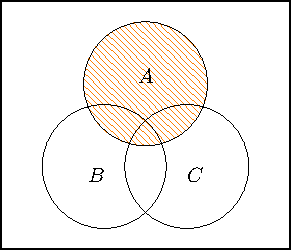
\includegraphics[width=1\linewidth]{math1710_files/figure-latex/dist1-1} \end{center}

~

\begin{center}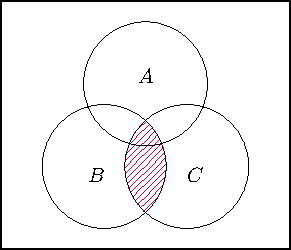
\includegraphics[width=1\linewidth]{math1710_files/figure-latex/dist2-1} \end{center}

~

\begin{center}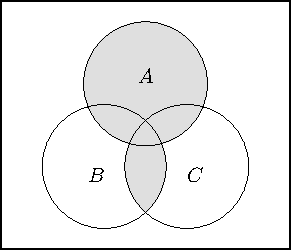
\includegraphics[width=1\linewidth]{math1710_files/figure-latex/dist3-1} \end{center}

The left-hand figure is \(\color{orange}{A}\), the middle figure is \(\color{purple}{B\cap C}\), and the right-hand figure is union of these, \(A\cup (B\cap C)\).

Then for the right-hand side of the law, we have:

\begin{center}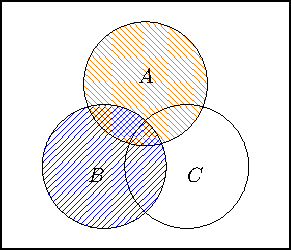
\includegraphics[width=1\linewidth]{math1710_files/figure-latex/dist4-1} \end{center}

~

\begin{center}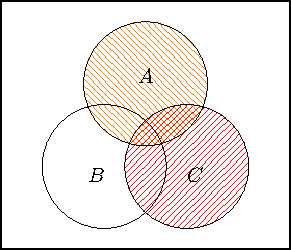
\includegraphics[width=1\linewidth]{math1710_files/figure-latex/dist5-1} \end{center}

~

\begin{center}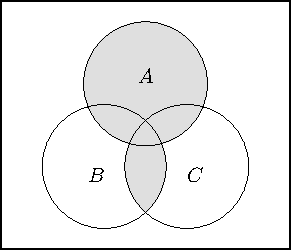
\includegraphics[width=1\linewidth]{math1710_files/figure-latex/dist6-1} \end{center}

The left-hand figure is \(\color{orange}{A} \cup \color{blue}{B}\), the middle figure is \(\color{orange}{A}\cup \color{red}{C}\), and the right-hand figure is intersection of these, \((A\cup B)\cap (A\cup C)\).

We see that the areas shaded in two right-hand figures are the same, so it is indeed the case that
\(A\cup (B\cap C) = (A\cup B)\cap (A\cup C)\).

\section*{Summary}\label{summary-L03}
\addcontentsline{toc}{section}{Summary}

\begin{itemize}
\tightlist
\item
  A sample space \(\Omega\) is a set representing all possible sample outcomes.
\item
  An event is a subset of \(\Omega\).
\item
  For events \(A\) and \(B\), we also have the complement ``not \(A\)'' \(A^\mathsf{c}\), the intersection ``\(A\) and \(B\)'' \(A \cap B\), and the union ``\(A\) or \(B\)'' \(A \cup B\).
\end{itemize}

\textbf{Recommended reading:}

\begin{itemize}
\tightlist
\item
  \href{https://leeds.primo.exlibrisgroup.com/permalink/44LEE_INST/13rlbcs/alma991013131349705181}{Stirzaker, \emph{Elementary Probability}}, Sections 1.1 and 1.2 (plus optionally Chapter 0).
\item
  \href{https://leeds.primo.exlibrisgroup.com/permalink/44LEE_INST/13rlbcs/alma991002938669705181}{Grimmett and Welsh, \emph{Probability}}, Sections 1.1 and 1.2.
\end{itemize}

\chapter{Expectation and covariance}\label{L14-covariance}

\newcommand{\Cov}{\operatorname{Cov}}
\newcommand{\Corr}{\operatorname{Corr}}

\section{Expectation of sums and products}\label{sum-product}

When we have multiple random variables, we might be interested in functions of those multiple random variables -- for example their sum or their product. It's often possible to find out about the whole distribution of a sum, product, or function of the variables -- see MATH2715 Statistical Methods for more on this -- but here we will just look at their expectations and, later, variances.

\begin{theorem}
\protect\hypertarget{thm:linearity2}{}\label{thm:linearity2}

Let \(X\) and \(Y\) be two random variables with joint probability mass function \(p_{X,Y}\). Then

\begin{enumerate}
\def\labelenumi{\arabic{enumi}.}
\tightlist
\item
  \(\mathbb Eg(X,Y) = \displaystyle\sum_{x,y} g(x,y) p_{X,Y}(x,y)\).
\item
  \textbf{(Linearity of expectation, 2)} \(\mathbb E(X + Y) = \mathbb EX + \mathbb EY\), regardless of whether \(X\) and \(Y\) are independent or not.
\item
  If \(X\) and \(Y\) are independent, then \(\mathbb EXY = \mathbb EX \times \mathbb EY\).
\end{enumerate}

\end{theorem}

If we put the second point here together with the other result of linearity of expectation (Theorem \ref{thm:linearity1}) then we get the general rule
\[ \mathbb E(aX + bY + c) = a\,\mathbb EX + b \,\mathbb EY + c , \]
and this holds whether or not \(X\) and \(Y\) are independent.

\begin{proof}
Part 1 is just the law of the unconscious statistician for the random variable \((X,Y)\), and the same proof holds.

For part 2, we have
\begin{align*}
\mathbb E(X + Y) &= \sum_{x,y} (x + y)p_{X,Y}(x,y) \\
  &= \sum_{x,y} x\,p_{X,Y}(x,y) + \sum_{x,y} y\,p_{X,Y}(x,y) \\
  &= \sum_x x \sum_y p_{X,Y}(x,y) + \sum_y y \sum_x p_{X,Y}(x,y)
\end{align*}
But summing a joint PMF over one of the variables gives the marginal PMF; so \(\sum_y p_{X,Y}(x,y) = p_X(x)\) and \(\sum_x p_{X,Y}(x,y) = p_Y(y)\). So this gives
\begin{align*}
\mathbb E(X + Y) &= \sum_x x\, p_X(x) + \sum_y y\,p_Y(y) \\
&= \mathbb EX + \mathbb EY .
\end{align*}

For part 3, if \(X\) and \(Y\) are independent, then \(p_{X,Y}(x,y) = p_X(x) \, p_Y(y)\). Therefore,
\begin{align*}
\mathbb EXY &= \sum_{x,y} xy p_{X,Y}(x,y) \\
  &= \sum_x \sum_y xy p_X(x) p_Y(y) \\
  &= \sum_x x p_X(x) \sum_y y p_Y(y) \\
  &= \mathbb EX \times \mathbb EY,
\end{align*}
as required.
\end{proof}

\begin{example}
Let \(X_1, X_2, \dots, X_n\) be IID \(\text{Bern}(p)\) random variables. We know that \(\mathbb EX_1 = p\) and \(\operatorname{Var}(X_1) = p(1-p)\).

Now let \(Y = X_1 + X_2 + \cdots + X_n\). Since each \(X_i\) indicates whether or not trial \(i\) was a success, this means \(Y\) counts the number of successes in \(n\) trials. This is a binomial random variable, \(Y \sim \text{Bin}(n,p)\).

We can use this structure to calculate
\[ \mathbb EY = \mathbb E(X_1 + \cdots + X_n) = n \mathbb EX_1 = np . \]

This has proved the expectation of the binomial distribution from Lecture 11. (Note that this would hold even if the trials weren't independent.)
\end{example}

\section{Covariance}\label{covariance}

If we are interested at how two random variables vary together, we need to look at the covariance.

\begin{definition}
Let \(X\) and \(Y\) be two random variables with expectations \(\mathbb EX =\mu_X\) and \(\mathbb EY = \mu_Y\) respectively. Then their \textbf{covariance} is
\[ \operatorname{Cov}(X,Y) = \mathbb E(X - \mu_X)(Y - \mu_Y) . \]
\end{definition}

In the least surprising result of this whole module, we also have a computational formula to go along with this definitional formula.

\begin{theorem}
Let \(X\) and \(Y\) be two random variables with expectations \(\mu_X\) and \(\mu_Y\) respectively. Then their covariance can also be calculated as
\[ \operatorname{Cov}(X,Y) = \mathbb EXY - \mu_X\, \mu_Y . \]
\end{theorem}

\begin{proof}
Exactly as we've done many times before, we have
\begin{align*}
\operatorname{Cov}(X,Y) &= \mathbb E(X - \mu_X)(Y - \mu_Y) \\
&= \mathbb E(XY - X\,\mu_Y - \mu_X\, Y + \mu_X\,\mu_Y) \\
&= \mathbb EXY  - \mu_Y \,\mathbb EX - \mu_X \,\mathbb EY + \mu_X \, \mu_Y \\
&= \mathbb EXY - \mu_X \, \mu_Y - \mu_X \, \mu_Y + \mu_X \, \mu_Y \\
&= \mathbb EXY - \mu_X \, \mu_Y ,
\end{align*}
and we're done.
\end{proof}

\begin{example}
We continue with our coin-tossing example from the previous lecture, where \(X\) is the number of Heads in the first two coin tosses and \(Y\) the number of Heads in the first three coin tosses.

We know that \(X \sim \text{Bin}(2, \frac12)\), so \(\mu_X = 1\), and \(Y \sim \text{Bin}(3, \frac12)\), so \(\mu_Y = 1.5\). To find the covariance using the computational formula, we also need \(\mathbb EXY\), which is
\begin{align*}
\mathbb EXY &= \sum_{x,y} xy\, p_{X,Y}(x,y) \\
  &= 0\times 0\times p_{X,Y}(0,0) + 0 \times 1 \times p_{X,Y}(0,1) + \cdots + 2\times 3 \times p_{X,Y}(2,3) \\
  &= 0 \times \tfrac18 + 0 \times \tfrac18 + \cdots + 6 \times \tfrac18 \\
  &= 2.
\end{align*}
Hence the covariance is
\[ \operatorname{Cov}(X,Y) = \mathbb EXY - \mu_X\mu_Y = 2 - 1 \times 1.5 = 0.5 .\]
\end{example}

A very important fact is the following.

\begin{theorem}
If \(X\) and \(Y\) are independent, then \(\operatorname{Cov}(X,Y) = 0\).
\end{theorem}

Be careful not to get this the wrong way around: if \(\operatorname{Cov}(X,Y) = 0\) it doesn't necessarily mean that \(X\) and \(Y\) are independent.

To use the \href{https://www.varsitytutors.com/hotmath/hotmath_help/topics/converse-inverse-contrapositive}{``contrapositive''} (which is allowed!), in our example, we have \(\operatorname{Cov}(X,Y) \neq 0\), which means that \(X\) and \(Y\) are not independent -- confirming what we already knew.

\begin{proof}
Recall from Theorem \ref{thm:linearity2} that if \(X\) and \(Y\) are independent, we have \(\mathbb EXY = \mathbb EX \times \mathbb EY = \mu_X \, \mu_Y\). Then from the computational formula, we have
\[ \operatorname{Cov}(X,Y) = \mathbb EXY - \mu_X\,\mu_Y = \mu_X\,\mu_Y - \mu_X\,\mu_Y = 0, \]
and we are done.
\end{proof}

Here are some more important properties of the covariance.

\begin{theorem}

Let \(X\), \(Y\) and \(Z\) be random variables. Then

\begin{enumerate}
\def\labelenumi{\arabic{enumi}.}
\tightlist
\item
  \(\operatorname{Cov}(X,Y) = \operatorname{Cov}(Y,X)\);
\item
  \(\operatorname{Cov}(X,X) = \operatorname{Var}(X)\);
\item
  \(\operatorname{Cov}(aX, Y) = a\,\operatorname{Cov}(X,Y)\);
\item
  \(\operatorname{Cov}(X + b, Y) = \operatorname{Cov}(X,Y)\);
\item
  \(\operatorname{Cov}(X + Y, Z) = \operatorname{Cov}(X, Z) + \operatorname{Cov}(Y,Z)\).
\end{enumerate}

\end{theorem}

\begin{proof}
Part 1 and 2 are immediate from the definition.

Parts 3, 4 and 5 are quite similar. We'll do part 5 here, and you can do parts 3 and 4 on \hyperref[P4]{Problem Sheet 4}.

For part 5, note that \(\mathbb E(X + Y) = \mu_X + \mu_Y\) by linearity of expectation. Hence
\begin{align*}
\operatorname{Cov}(X + Y, Z)
  &= \mathbb E \big((X + Y) - (\mu_X + \mu_Y)\big)(Z - \mu_Z) \\
  &= \mathbb E \big((X - \mu_X) + (Y - \mu_Y)\big)(Z - \mu_Z) \\
  &= \mathbb E \big((X - \mu_X)(Z - \mu_Z) + (Y - \mu_Y) (Z - \mu_Z) \big) \\
  &= \mathbb E (X - \mu_X)(Z - \mu_Z) + \mathbb E  (Y - \mu_Y) (Z - \mu_Z) \\
  &= \operatorname{Cov}(X,Z) + \operatorname{Cov}(Y,Z) ,
\end{align*}
as required.
\end{proof}

\begin{example}
We could calculate the covariance in our coin-tossing example a different way, by noting that \(Y = X + Z\), where \(Z \sim \text{Bern}(\frac12)\) represents the third coin toss and is independent of \(X\). Then we have
\[
\operatorname{Cov}(X,Y) = \operatorname{Cov}(X, X + Z) = \operatorname{Cov}(X, X) + \operatorname{Cov}(X, Z)
= \operatorname{Var}(X) + 0 = \operatorname{Var}(X) ,\]
where we used \(\operatorname{Cov}(X, Z) = 0\) since \(X\) and \(Z\) are independent.
We already know that \(\operatorname{Var}(X) = 2 \times \tfrac12 \times (1 - \tfrac12) = \tfrac12\) because \(X \sim \text{Bin}(2, \frac12)\). So \(\operatorname{Cov}(X,Y) = \frac12\),
matching our previous calculation.
\end{example}

Now that we know some facts about the covariance, we can calculate the variance of a sum.

\begin{theorem}
Let \(X\) and \(Y\) be two random variables. Then
\[ \operatorname{Var}(X + Y) = \operatorname{Var}(X) + 2\operatorname{Cov}(X,Y) + \operatorname{Var}(Y) . \]

If \(X\) and \(Y\) are independent, then
\[ \operatorname{Var}(X + Y) = \operatorname{Var}(X) + \operatorname{Var}(Y) . \]
\end{theorem}

It's easy to forget the conditions for the following two facts:

\begin{itemize}
\tightlist
\item
  \(\mathbb E(X + Y) = \mathbb EX + \mathbb EY\) regardless of whether \(X\) and \(Y\) are independent or not.
\item
  \(\operatorname{Var}(X+Y) = \operatorname{Var}(X) + \operatorname{Var}(Y)\) if \(X\) and \(Y\) are independent.
\end{itemize}

\begin{proof}
For the main part of the proof, we start with the definition of variance. By linearity of expectation, we have \(\mathbb E(X + Y) = \mu_X + \mu_Y\). So
\begin{align*}
\operatorname{Var}(X + Y) &= \mathbb E\big((X + Y) - (\mu_X + \mu_Y)\big)^2 \\
  &= \mathbb E \big((X - \mu_X) + (Y - \mu_Y) \big)^2 \\
  &= \mathbb E \big( (X - \mu_X)^2 + 2(X - \mu_X)(Y - \mu_Y) + (Y - \mu_Y)^2\big) \\
  &= \mathbb E(X - \mu_X)^2 + 2 \mathbb E(X - \mu_X)(Y - \mu_Y) + \mathbb E (Y - \mu_Y)^2 \\
  &= \operatorname{Var}(X) + 2\operatorname{Cov}(X,Y) + \operatorname{Var}(Y) ,
\end{align*}
where we used the linearity of expectation.

For the second part, recall that is \(X\) and \(Y\) are independent, then \(\operatorname{Cov}(X,Y) = 0\).
\end{proof}

\begin{example}
Returning to the ``binomial as a sum of Bernoullis'' example, we have
\[ \operatorname{Var}(Y) = \operatorname{Var}(X_1 + \cdots X_n) = n\operatorname{Var}(X_1) = np(1-p) . \]
Here we used that the \(X_i\) are independent (the first I in ``IID'').
\end{example}

\section{Correlation}\label{correlation}

It can sometimes be useful to ``normalise'' the covariance, by dividing through by the individual standard deviations. This gives a measurement of the linear relationship between two random variables.

\begin{definition}
Let \(X\) and \(Y\) be two random variables. Then the \textbf{correlation} between \(X\) and \(Y\) is
\[ \operatorname{Corr}(X,Y) = \frac{\operatorname{Cov}(X,Y)} {\sqrt{\operatorname{Var}(X)\,\operatorname{Var}(Y)}} . \]
\end{definition}

As with the sample correlation \(r_{xy}\) from Section 1, the correlation is a number between \(-1\) and \(+1\), where values near \(+1\) mean that large values of \(X\) and large values of \(Y\) are likely to occur together, while values near \(-1\) mean that large values of \(X\) and small values of \(Y\) are likely to occur together.

Recall that, if \(X\) and \(Y\) are independent, then \(\operatorname{Cov}(X,Y) = 0\). Hence it follows that if \(X\) and \(Y\) are independent, then \(\operatorname{Corr}(X,Y) = 0\) also.

\begin{example}
For the coin-tossing again, we have
\[ \operatorname{Corr}(X,Y) = \frac{\operatorname{Cov}(X,Y)} {\sqrt{\operatorname{Var}(X)\,\operatorname{Var}(Y)}} = \frac{\frac12}{\sqrt{\frac12 \times \frac34}} = \sqrt{\tfrac23} = 0.816 .    \]
\end{example}

\section*{Summary}\label{summary-L14}
\addcontentsline{toc}{section}{Summary}

\begin{itemize}
\tightlist
\item
  \(\mathbb E(X + Y) = \mathbb EX + \mathbb EY\)
\item
  The covariance is \(\operatorname{Cov}(X,Y) = \mathbb E(X - \mu_X)(Y - \mu_Y) = \mathbb EXY - \mu_X \,\mu_Y\).
\item
  \(\operatorname{Var}(X + Y) = \operatorname{Var}(X) + 2\operatorname{Cov}(X,Y) + \operatorname{Var}(Y)\); or if \(X\) and \(Y\) are independent, then \(\operatorname{Var}(X + Y) = \operatorname{Var}(X) + \operatorname{Var}(Y)\).
\end{itemize}

\textbf{Recommended reading:}

\begin{itemize}
\tightlist
\item
  \href{https://leeds.primo.exlibrisgroup.com/permalink/44LEE_INST/13rlbcs/alma991013131349705181}{Stirzaker, \emph{Elementary Probability}}, Sections 5.3.
\item
  \href{https://leeds.primo.exlibrisgroup.com/permalink/44LEE_INST/13rlbcs/alma991002938669705181}{Grimmett and Welsh, \emph{Probability}}, Section 3.2 and 3.4.
\end{itemize}

\commtrue

\chapter*{Solutions and group feedback}\label{solutions}
\addcontentsline{toc}{chapter}{Solutions and group feedback}

This page has the solutions to all the non-assessed questions on Problem Sheet 1. Solutions are added after all tutorials on a Problem Sheet have finished.

Solutions to assessed questions are available on Minerva in the ``Assessments and Feedback'' tab, from one week after the deadline.

There are many ways you get feedback on this module, both group feedback (feedback that is generally relevant to many people) and individual feedback (feedback based specifically on your own approach to the work).

\begin{itemize}
\item
  You will have received both individual and group spoken feedback in your tutorial (the more you speak up in your tutorial, the more individualised the feedback you get in return).
\item
  These solutions include group written feedback on common issues for the class.
\item
  Most importantly, when your work on assessed questions is marked, individual written feedback will be given via the Gradescope site. It is very important that you read that feedback.
\item
  Finally, students who would like even more feedback can discuss their work with me in the ``office hours'' drop-in sessions.
\end{itemize}

\section*{Problem Sheet 1}\label{P1-solutions}
\addcontentsline{toc}{section}{Problem Sheet 1}

\subsection*{A: Short questions}\label{P1-short-solutions}
\addcontentsline{toc}{subsection}{A: Short questions}

\begin{Shaded}
\begin{Highlighting}[]
\KeywordTok{\textbackslash{}begin}\NormalTok{\{}\ExtensionTok{tikzpicture}\NormalTok{\}[line width=0.25pt, scale=0.8]}

\KeywordTok{\textbackslash{}begin}\NormalTok{\{}\ExtensionTok{scope}\NormalTok{\} }
    \FunctionTok{\textbackslash{}fill}\NormalTok{  [red!25] (2,2) circle (1.5); }
    \FunctionTok{\textbackslash{}fill}\NormalTok{  [red!25] (4,2) circle (1.5); }
\KeywordTok{\textbackslash{}end}\NormalTok{\{}\ExtensionTok{scope}\NormalTok{\}}

\FunctionTok{\textbackslash{}draw}\NormalTok{[thick] (0,0) rectangle (6,4);}
\FunctionTok{\textbackslash{}draw}\NormalTok{ (6.3,3.8) node \{}\SpecialStringTok{$}\SpecialCharTok{\textbackslash{}Omega}\SpecialStringTok{$}\NormalTok{\};}
\FunctionTok{\textbackslash{}draw}\NormalTok{ (2,2) circle (1.5); }\FunctionTok{\textbackslash{}draw}\NormalTok{ (1.6,2.0) node \{}\SpecialStringTok{$Abcd$}\NormalTok{\};}
\FunctionTok{\textbackslash{}draw}\NormalTok{ (4,2) circle (1.5); }\FunctionTok{\textbackslash{}draw}\NormalTok{ (4.4,2.0) node \{}\SpecialStringTok{$Bxyz$}\NormalTok{\};}

\KeywordTok{\textbackslash{}end}\NormalTok{\{}\ExtensionTok{tikzpicture}\NormalTok{\}}
\end{Highlighting}
\end{Shaded}

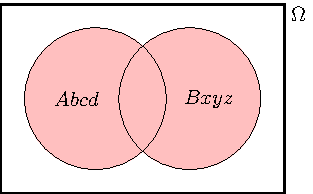
\includegraphics{math1710_files/figure-latex/amandatest44-1.pdf}

\textbf{A1.} Consider again the ``number of Skittles in each packet'' data from Example 1.1.
\[ 59, \ 59, \ 59, \ 59, \ 60, \ 60, \ 60, \ 61, \ 62, \ 62, \ 62, \ 63, \ 63 .\]

\textbf{(a)} Calculate the mean number of Skittles in each packet.

\begin{myanswers}
\emph{Solution.} This was in the notes:
\[ \bar x = \frac{1}{13} (59 + 59 + \cdots + 63) =  \frac{789}{13} = 60.6923\dots \approx 60.7 .\]

\end{myanswers}

\textbf{(b)} Calculate the sample variance using the definitional
formula.

\begin{myanswers}
\emph{Solution.}
\begin{align*}
s_x^2 &= \frac{1}{13 - 1} \left( (59 - 60.7)^2 + (59 - 60.7)^2 + \cdots + (63 - 60.7)^2 \right) \\
      &= \frac{1}{12} (2.86 + 2.86 + \cdots + 5.33) \\
      &= \frac{1}{12} \times 28.77 \\
      &= 2.40
\end{align*}

\end{myanswers}

\textbf{(c)} Calculate the sample variance using the computational formula.

\begin{myanswers}
\emph{Solution.}
\begin{align*}
s_x^2 &= \frac{1}{13 - 1} \left( (59^2 + 59^2 + \cdots + 63^2) - 13 \times 60.6923^2)\right) \\
      &= \frac{1}{12} (47915 - 47886.2) \\
      &= 2.40
\end{align*}

\textbf{Group feedback:} With the computational formula, the value \(\sum_i x_i^2 - n \bar{x}^2\) is typically a fairly small number given as the difference between two very big numbers \(\sum_i x_i^2\) and \(n \bar x^2\). This means you have to get the two big numbers very precise, to ensure the cancellation happens correctly; in particular, make sure you use plenty of decimal places of accuracy in \(\bar x\).

\end{myanswers}

\textbf{(d)} Out of (b) and (c), which calculation did you find easier, and why?

\begin{myanswers}
\emph{Solution.} The computational formula required fewer presses of the calculator buttons, because \(\sum_i x_i^2\) is fewer button-presses than \(\sum_i (x_i - \bar x)^2\), where you have to subtract the means before squaring.

On the other hand, the expression inside the brackets of the computational formula is a fairly small number given as the difference of two very large numbers, so it was necessary to use lots of decimal places of accuracy in \(\bar x\) to make sure the second large number was accurate and therefore that the subtraction cancelled correctly.

\textbf{Group feedback:} Many different answers for (d) are fine provided you give a justification.

\end{myanswers}

\textbf{A2.} Consider the following data sets of the age of elected politicians on a local council. (The ``18--30'' bin, for example, means from one's
18th birthday to the moment before one's 30th birthday, so lasts 12 years.)

\begin{longtable}[]{@{}
  >{\centering\arraybackslash}p{(\columnwidth - 6\tabcolsep) * \real{0.2537}}
  >{\centering\arraybackslash}p{(\columnwidth - 6\tabcolsep) * \real{0.1642}}
  >{\centering\arraybackslash}p{(\columnwidth - 6\tabcolsep) * \real{0.2985}}
  >{\centering\arraybackslash}p{(\columnwidth - 6\tabcolsep) * \real{0.2836}}@{}}
\toprule\noalign{}
\begin{minipage}[b]{\linewidth}\centering
Age (years)
\end{minipage} & \begin{minipage}[b]{\linewidth}\centering
Frequency
\end{minipage} & \begin{minipage}[b]{\linewidth}\centering
Relative frequency
\end{minipage} & \begin{minipage}[b]{\linewidth}\centering
Frequency density
\end{minipage} \\
\midrule\noalign{}
\endhead
\bottomrule\noalign{}
\endlastfoot
18--30 & 1 & & \\
30--40 & 2 & & \\
40--45 & 4 & & \\
45--50 & 5 & & \\
50--60 & 6 & & \\
60--80 & 2 & & \\
\textbf{Total} & 20 & 1 & --- \\
\end{longtable}

\textbf{(a)} Complete the table by filling in the relative frequency and
frequency densities.

\begin{myanswers}

\emph{Solution.}

\begin{longtable}[]{@{}
  >{\centering\arraybackslash}p{(\columnwidth - 6\tabcolsep) * \real{0.2537}}
  >{\centering\arraybackslash}p{(\columnwidth - 6\tabcolsep) * \real{0.1642}}
  >{\centering\arraybackslash}p{(\columnwidth - 6\tabcolsep) * \real{0.2985}}
  >{\centering\arraybackslash}p{(\columnwidth - 6\tabcolsep) * \real{0.2836}}@{}}
\toprule\noalign{}
\begin{minipage}[b]{\linewidth}\centering
Age (years)
\end{minipage} & \begin{minipage}[b]{\linewidth}\centering
Frequency
\end{minipage} & \begin{minipage}[b]{\linewidth}\centering
Relative frequency
\end{minipage} & \begin{minipage}[b]{\linewidth}\centering
Frequency density
\end{minipage} \\
\midrule\noalign{}
\endhead
\bottomrule\noalign{}
\endlastfoot
18--30 & 1 & 0.05 & 0.0042 \\
30--40 & 2 & 0.1 & 0.01 \\
40--45 & 4 & 0.2 & 0.04 \\
45--50 & 5 & 0.25 & 0.05 \\
50--60 & 6 & 0.3 & 0.03 \\
60--80 & 2 & 0.1 & 0.005 \\
\textbf{Total} & 20 & 1 & --- \\
\end{longtable}

\end{myanswers}

\textbf{(b)} What is the median age bin?

\begin{myanswers}
\emph{Solution.} The 10th- and 11th-largest observations are both in the 45--50 bin, which is therefore the median bin.

\end{myanswers}

\textbf{(c)} What is the modal age bin?

\begin{myanswers}
\emph{Solution.} The bin with the largest frequency density is 45--50, which is therefore the modal bin.

\textbf{Group feedback:} Remember that the modal bin is the one with the largest frequency \emph{density}, not necessarily the bin with the highest frequency.

\end{myanswers}

\textbf{(d)} Calculate (the standard approximation of) the mean age of the politicians.

\begin{myanswers}
\emph{Solution.} Pretending that each person is in the centre of their bin, we have
\[ \bar x = \frac{1}{20} (1\times24 + 2\times 35 + \cdots + 2 \times 65) = \frac{971.9}{20} = 48.6 . \]

\end{myanswers}

\textbf{A3.} Consider the two datasets illustrated by the boxplots below. Write down some differences between the two datasets.

\begin{myanswers}
\emph{Solution.} Some answers could be:

\begin{itemize}
\tightlist
\item
  The median and inter-quartile range of Dataset 2 appear to be very slightly larger than those in Dataset 1, although the differences are very small and might not be important in real life.
\item
  Dataset 2 has a few outliers; Dataset 1 has none.
\item
  While Dataset 1 is fairly ``balanced'' either side of the median, Dataset 2 shows what statisticians call a ``positive skew'': the data above the median is much more spread out than the data below the median.
\end{itemize}

\textbf{Group feedback:}
You can probably think of other answers.

\end{myanswers}

\subsection*{B: Long questions}\label{P1-long-solutions}
\addcontentsline{toc}{subsection}{B: Long questions}

--\textgreater{}
\#\# Problem Sheet 2 \{\#P2-solutions .unnumbered\}

\subsection*{A: Short questions}\label{P2-short-solutions}
\addcontentsline{toc}{subsection}{A: Short questions}

\textbf{A1.} Suppose you toss a coin 4 times.

\textbf{(a)} What would you suggest for a sample space \(\Omega\) \textbf{(i)} if you only care about the total number of heads; \textbf{(ii)} if you care about the result of each coin toss?

\textbf{(b)} For each of the cases in part (a), what is \(|\Omega|\)?

\begin{myanswers}
\emph{Solution.}

\textbf{(i)} We can take \(\Omega = \{0,1,2,3,4\}\), with \(|\Omega| = 5\).

\textbf{(ii)} Here, \(\Omega = \{ \text{HHHH}, \text{HHHT}, \text{HHTH},\dots, \text{TTTT} \}\) should be the set of all sequences of four ``H''s or ``T''s. So here, \(|\Omega| = 2^4 = 16\).

\end{myanswers}

\textbf{A2.} Let \(A\), \(B\) and \(C\) be events in a sample space \(\Omega\). Write the following events using only \(A\), \(B\), \(C\) and the complement, intersection, and union operations.

\textbf{(a)} \(C\) happens but \(A\) doesn't.

\begin{myanswers}
\emph{Solution.} This is ``\(C\) and not \(A\)'': \(C\cap A^{\mathsf{c}}\).

\end{myanswers}

\textbf{(b)} At least one of \(A\), \(B\) and \(C\) happens.

\begin{myanswers}
\emph{Solution.} This is simply the union \(A \cup B\cup C\).

\end{myanswers}

\textbf{(c)} Exactly one of \(B\) or \(C\) happens.

\begin{myanswers}
\emph{Solution.} One way to write this is to split it up as ``\,`\(B\) but not \(C\)' or `\(C\) but not \(B\)'\,'', which is \((B \cap C^{\mathsf{c}}) \cup (B^{\mathsf{c}} \cap C)\).

An alternative is to split it up as ``\,`\(B\) or \(C\)' but not `both \(B\) and \(C\)'\,'', which is \((B \cup C) \cap (B\cap C)^{\mathsf{c}}\).

You can check these are equal by (for example) using De Morgan's law and the distributive law to expand out the second version.

\end{myanswers}

\textbf{(d)} Exactly two of \(A\), \(B\) and \(C\) happens.

\begin{myanswers}
\emph{Solution.} I would split this up into ``\(A\) and \(B\) but not \(C\)'', ``\(A\) and \(C\) but not \(B\)'', and ``\(B\) and \(C\) but not \(A\)'' and take the union. This gives
\[  (A \cap B \cap C^{\mathsf{c}}) \cup (A \cap B^{\mathsf{c}} \cap C) \cup (A^{\mathsf{c}} \cap B \cap C) . \]
There are other equivalent formulations.

\end{myanswers}

\textbf{A3.} What is the value of the following expressions?

\textbf{(a)} \(6!\)

\begin{myanswers}
\emph{Solution.}
\[ 6! = 6 \times 5 \times 4 \times 3 \times 2 \times 1 = 720. \]

\end{myanswers}

\textbf{(b)} \(8^4\)

\begin{myanswers}
\emph{Solution.}
\[ 8^4 = 8 \times 8 \times 8 \times 8 = 4096 \]

\end{myanswers}

\textbf{(c)} \({8}^{\underline{4}}\)

\begin{myanswers}
\emph{Solution.}
\[ {8}^{\underline{4}} = 8 \times 7 \times 6 \times 5 = 1680 \]

\end{myanswers}

\textbf{(d)} \({\displaystyle \binom{10}{4}}\)

\begin{myanswers}
\emph{Solution.}
\[ \binom{10}{4} = \frac{10 \times 9 \times 8 \times 7}{4\times 3\times 2\times 1} = 210 \]

\end{myanswers}

\textbf{A4.} An urn contains 4 red balls and 6 blue balls. Two balls are drawn from the urn. What is the probability that both balls are red, if the balls are drawn \textbf{(a)} with replacement; \textbf{(b)} without replacement?

\begin{myanswers}
\emph{Solution.}

\textbf{(a)} There are \(|\Omega| = 10^2 = 100\) ways to draw two balls with replacement. There are \(|A| = 4^2=16\) ways to draw two red balls. So
\(\mathbb P(A) = \frac{16}{100} = 0.16\).

\textbf{(b)} There are \(|\Omega| = {10}^{\underline{2}} = 10 \times 9 = 90\) ways to draw two balls without replacement. There are \(|A| = {4}^{\underline{2}} = 4 \times 3 = 12\) to draw two red balls. So
\(\mathbb P(A) = \frac{12}{90} = \frac{2}{15} = 0.133\).

\end{myanswers}

\subsection*{B: Long questions}\label{P2-long-solutions}
\addcontentsline{toc}{subsection}{B: Long questions}

\textbf{B1.} Starting from just the three probability axioms, prove the following statements:

\textbf{(a)} \(\mathbb P(\varnothing) = 0\).

\begin{myanswers}
\emph{Solution.} Let \(A\) be any event (such as \(A = \varnothing\) or \(A = \Omega\), for example). Then \(A \cup \varnothing = A\), and the union is disjoint -- since \(\varnothing\) contains no sample points, it certainly can't contain any sample points that are also in \(A\). Then applying Axiom 3, we get \(\mathbb P(A) + \mathbb P(\varnothing) = \mathbb P(A)\). Subtracting \(\mathbb P(A)\) from both sides gives the result.

\emph{Alternatively}, if you prove part (b) first, you can apply that with \(A = \varnothing\). Since \(\varnothing^\mathsf{c}= \Omega\) and Axiom 2 tells us that \(\mathbb P(\Omega) = 1\), the result follows.

\textbf{Group feedback:} With this, and most ``prove from the axioms'' questions, the key is to find a relevant disjoint union, which then allows us to use Axiom 3. So if we can find \(C = A \cup B\) as a disjoint union (hopefully containing some events relevant to the question at hand), Axiom 3 allows us to write \(\mathbb P(C) = \mathbb P(A) + \mathbb P(B)\).

\end{myanswers}

\textbf{(b)} \(\mathbb P(A^\mathsf{c}) = 1 - \mathbb P(A)\).

\begin{myanswers}
\emph{Solution.} A very useful and relevant disjoint union is \(A \cup A^\mathsf{c}= \Omega\). Applying Axiom 3 gives us \(\mathbb P(A) + \mathbb P(A^\mathsf{c}) = \mathbb P(\Omega)\). But Axiom 2 tells us that \(\mathbb P(\Omega) = 1\), so \(\mathbb P(A) + \mathbb P(A^\mathsf{c}) = 1\). Rearranging gives the result.

\end{myanswers}

\textbf{B2.} In this question, you will have to use the standard two-event form of the addition rule for unions
\[ \mathbb P(A \cup B) = \mathbb P(A) + \mathbb P(B) - \mathbb P(A \cap B) . \]

\textbf{(a)} Using the two-event addition rule, show that
\[ \mathbb P(C \cup D \cup E) = \mathbb P(C) + \mathbb P(D \cup E) - \mathbb P\big(C \cap (D \cup E)\big).  \]

\begin{myanswers}
\emph{Solution.} As with the Cauchy--Schwarz question from Problem Sheet 1, the key is to make a good choice for what \(A\) and \(B\) should be. This time, \(A = C\) and \(B = D \cup E\) will work well, since \(C \cup (D \cup E) = C \cup D \cup E\). (You can call this ``associativity'', if you like.) Making that substitution immediately gives us
\[ \mathbb P(C \cup D \cup E) = \mathbb P(C) + \mathbb P(D \cup E) - \mathbb P\big(C \cap (D \cup E)\big) ,  \]
as required.

\end{myanswers}

\textbf{(b)} Using your result from part (a), the two-event addition rule, the distributive law, and the two-event addition rule again, prove the three-event form of the addition rule for unions:
\[
  \mathbb P(C \cup D \cup E) = \mathbb P(C) + \mathbb P(D) + \mathbb P(E) 
  - \mathbb P(C \cap D) - \mathbb P(C \cap E) - \mathbb P(D \cap E) + \mathbb P(C \cap D \cap E) .
\]

\begin{myanswers}
\emph{Solution.}
Let's take the three terms on the right of the equation from part (a) separately.

The first term is \(\mathbb P(C)\), which is fine as it is.

The second term is \(\mathbb P(D \cup E)\). This is the probability of the union of two events, so we can use addition rule for the union of two events to get
\[ \mathbb P(D \cup E) = \mathbb P(D) + \mathbb P(E) - \mathbb P(D \cap E) . \]

The third term is \(\mathbb P\big(C \cap (D \cup E)\big)\). If we use the distributive law, as suggested in the question, we get \(C \cap (D \cup E) = (C \cap D) \cup (C\cap E)\), so we want to find \(\mathbb P\big((C \cap D) \cup (C\cap E)\big)\). But this is another union of two events again, this time with \(A = C \cap D\) and \(B = C \cap E\). So the two-event addition rule gives
\[ \mathbb P\big((C \cap D) \cup (C\cap E)\big) = \mathbb P(C \cap D) + \mathbb P(C \cap E) - \mathbb P(C \cap D \cap E) , \]
since \((C \cap D) \cap (C \cap E) = C \cap D \cap E\).

Finally, we put this all together, and get
\begin{align*}
  \mathbb P(C &\cup D \cup E) \\
  &= \mathbb P(C) + \big(\mathbb P(D) + \mathbb P(E) - \mathbb P(D \cap E)\big) - \big(\mathbb P(C \cap D) + \mathbb P(C \cap E) - \mathbb P(C \cap D \cap E)\big) \\
  &= \mathbb P(C) + \mathbb P(D) + \mathbb P(E) - \mathbb P(C \cap D) - \mathbb P(C \cap E) - \mathbb P(D \cap E) + \mathbb P(C \cap D \cap E) , 
\end{align*}
which is what we wanted.

\end{myanswers}

\textbf{B3.} Suppose we pick a number at random from the set \(\{1, 2, \dots, 2023\}\).

\textbf{(a)} What is the probability that the number is divisible by 5?

\begin{myanswers}

\emph{Solution.} The sample space is \(\Omega = \{1, 2, \dots, 2023\}\). Clearly \(|\Omega| = 2023\). The event in question is \(A = \{5, 10, \dots, 2020\}\) of numbers up to 2023 that are divisible by 5. Thus \(|A|\) is the largest integer no bigger than \(\frac{2023}{5} = 404.6\), which is 404, as this is how many times 5 ``goes into'' 2023. Hence
\[ \mathbb P(A) = \frac{|A|}{|\Omega|} = \frac{404}{2023} = 0.1997 , \]
just a tiny bit smaller than \(\frac{1}{5}\).

\textbf{Group feedback:} With these ``classical probability'' questions, the steps should always be:

\begin{enumerate}
\def\labelenumi{\arabic{enumi}.}
\tightlist
\item
  State clearly what the sample space \(\Omega\) is.
\item
  Count how many outcomes \(|\Omega|\) are in the sample space.
\item
  State clearly what the event \(A\) is.
\item
  Count how many outcomes \(|A|\) are in the event.
\item
  The desired probability is then \(\mathbb P(A) = |A|/|\Omega|\).
\end{enumerate}

\end{myanswers}

\textbf{(b)} What is the probability the number is divisible by 5 or by 7?

\begin{myanswers}
\emph{Solution.} With the same \(\Omega\) and \(A\), now let \(B\) be the numbers up to 2023 divisible by \(7\); so we're looking for \(\mathbb P(A \cup B)\). By the addition rule for unions, this is
\[ \mathbb P(A \cup B) = \mathbb P(A) + \mathbb P(B) - \mathbb P(A \cap B) . \]
We already know \(\mathbb P(A) = \frac{404}{2022}\), so need to find out \(\mathbb P(B)\) and \(\mathbb P(A \cap B)\).

This time, 7 goes into 2023 exactly, so \(|B|\) is \(\frac{2023}{7} = 289\). So
\[ \mathbb P(B) = \frac{|B|}{|\Omega|} = \frac{289}{2023} = \frac{1}{7}  . \]

Now, \(A \cap B\) is the set of numbers divisible by both 5 and 7, which is precisely the numbers divisible by their least common multiple \(5 \times 7 = 35\). Then \(|A \cap B|\) is \(\frac{2023}{35} = 57.8\) rounded down, so \(\mathbb P(A \cap B) = \frac{57}{2023}\).

So finally, we have
\[ \mathbb P(A \cup B) = \frac{404}{2023} + \frac{289}{2023} - \frac{57}{2023} = \frac{636}{2023} = 0.314 , \]
just a tiny bit larger than \(\frac{11}{35}\)

\end{myanswers}

\textbf{B4.} Eight friends are about to sit down at random at a round table. Find the probability that

\textbf{(a)} Ashley and Brook sit next to each other, with Chris directly opposite Brook;

\begin{myanswers}
\emph{Solution.}
Let \(\Omega\) be the sample space of ways the friends can sit around the table. This is an ordering problem, so \(|\Omega| = 8!\).

Let \(A\) be the event in the question. What is \(|A|\)? Well,

\begin{itemize}
\tightlist
\item
  Ashley can sit anywhere, so has 8 choices of seat.
\item
  Brook can sit either directly to Ashley's left or directly to Ashley's right, so has 2 choices of seat.
\item
  Chris must sit directly opposite Brook, so only has 1 choice of seat.
\item
  The remaining five friends can fill up the remaining seats however they like, so have 5, 4, 3, 2, and 1 choices respectively.
\end{itemize}

Hence \(|A| = 8 \times 2 \times 1 \times 5 \times 4 \times 3 \times 2 \times 1\). Thus we get
\[ \mathbb P(A) = \frac{|A|}{|\Omega|} = \frac{8 \times 2 \times 1 \times 5 \times 4 \times 3 \times 2 \times 1}{8 \times 7 \times 6 \times 5 \times 4 \times 3 \times 2 \times 1} = \frac{2 \times 1}{7 \times 6} = \frac{1}{21} . \]

\textbf{Group feedback:} As we have discussed more recently, after this Problem Sheet was assigned, often ``classical probability'' problems also can be equivalently solved by the step-by-step ``chain rule'' method. Can you use a chain rule argument to find the same answer as
\[ \mathbb P(A) = 1 \times \frac27 \times \frac16 \times 1 \times 1 \times 1 \times 1 \times 1 = \frac{1}{21} ? \]

\end{myanswers}

\textbf{(b)} neither Ashley, Brook nor Chris sit next to each other.

\begin{myanswers}
\emph{Solution.}
The sample space \(\Omega\) is as before. Let's count the outcomes in \(B\), the event in the question.

\begin{itemize}
\tightlist
\item
  Ashley can sit anywhere, so has 8 choices of seat.
\item
  Chris's number of choices will depend on where Brook sits, so we'll have to count Brook's and Chris's choices together:

  \begin{itemize}
  \tightlist
  \item
    Brook cannot sit next to Ashley.
  \item
    If Brook sits next-but-one to Ashley -- of which there are 2 choices -- then Chris has 3 choices: Chris cannot sit on the seat directly between Ashley and Brook, nor directly next to Ashley on the other side, nor directly next to Brook on the other side, leaving \(6-3=3\) choices.
  \item
    If Brook sits neither next nor next-but-one to Ashley -- of which there are 3 choices -- then Chris has 2 choices: he cannot sit to the right or left of Ashley, nor to the right or left of Brook, leaving \(6-4=2\) choices.
  \end{itemize}
\item
  The remaining friends have 5, 4, 3, 2, and 1 choices again.
\end{itemize}

Hence, \(|B| = 8 \times (2\times 3 + 3 \times 2) \times 5 \times 4 \times 3 \times 2 \times 1\). So
\[ \mathbb P(B) = \frac{|B|}{|\Omega|} = \frac{8 \times (2\times 3 + 3 \times 2) \times 5 \times 4 \times 3 \times 2 \times 1}{8 \times 7 \times 6 \times 5 \times 4 \times 3 \times 2 \times 1} = \frac{2\times 3 + 3 \times 2}{7 \times 6} = \frac{12}{42} = \frac{2}{7} .  \]

\emph{Alternatively}, in a previous year's tutorial, a MATH1710 student suggested to me the following rather elegant solution. Suppose the five other friends are already sat at a round table with five chairs. Ashley, then Brook, then Chris will each bring along their own chair, and push into one of the gaps between the friends.

Ashley has 5 gaps to choose from, then Brook will have 6 gaps (Ashley joining the table will have increased the number of gaps by 1), then Chris will have 7, so the total number of ways they can push in is \(|\Omega| = 5 \times 6 \times 7\).

To not sit next to each other, Ashley can push in any of the 5 gaps, Brook only has \(6 - 2 = 4\) choices (not in the gap directly to the left or right of Ashley), and Chris only has \(7 - 4 = 3\) choices (not in the gaps directly to the left or right of Ashley nor the gaps directly to the left or right of Brook -- these four gaps are distinct assuming Brook was not next to Ashley). Hence \(|B| = 5 \times 4 \times 3\), and we have
\[ \mathbb P(B) = \frac{5 \times 4 \times 3}{5 \times 6 \times 7} = \frac{4 \times 3}{6 \times 7} = \frac{12}{42} = \frac{2}{7}.  \]

\textbf{Group feedback:} Again, an equivalent answer can be derived using the step-by-step ``chain rule'' method.

\end{myanswers}

\textbf{B5.} A ``random digit'' is a number chosen at random from \(\{0, 1, \dots, 9\}\), each with equal probability. A statistician chooses \(n\) random digits (with replacement).

\textbf{(a)} For \(k = 0, 1, \dots, 9\), let \(A_k\) be the event that all the digits are \(k\) or smaller. What is the probability of \(A_k\), as a function of \(k\) and \(n\)?

\begin{myanswers}
\emph{Solution.}
The sample space is \(\Omega = \{0,1,\dots,9\}^n\), the set of length-\(n\) sequences of digits between \(0\) and \(9\). The number of these is \(|\Omega| = 10^n\), as there are 10 choices for each of the \(n\) digits.

The event \(A_k\) is \(\{0,1,\dots,k\}^n\), the set of length-\(n\) sequences of digits that are between \(0\) and \(k\). The number of these is \(|A_k| = (k+1)^n\). (Note that it's \(k+1\) because we're allowing 0 as well.)

Hence, the probability is
\[ \mathbb P(A_k) = \frac{|A_k|}{|\Omega|} = \frac{(k+1)^n}{10^n} . \]

\end{myanswers}

\textbf{(b)} Let \(B_k\) be the event that the largest digit chosen is equal to \(k\). By finding a relationship between \(B_k\), \(A_{k-1}\) and \(A_k\), or otherwise, show that
\[ \mathbb P(B_k) = \frac{(k+1)^n - k^n}{10^n} . \]

\begin{myanswers}
\emph{Solution.}
Consider the event \(A_k\) that all the digits are at most \(k\). Within \(A_k\), \emph{either} one or more of the digits equal \(k\), in which case that \(k\) is the largest digit and we are in \(B_k\); \emph{or} none of the digits equal \(k\), in which case they are all at most \(k-1\), and we are in \(A_{k-1}\). Only one of these two possibilitie can occur, so we have a disjoint union
\[ A_k = B_k \cup A_{k-1} . \]

Applying Axiom 3 to the disjoint union gives
\[ \mathbb P(A_k) = \mathbb P(B_k) + \mathbb P(A_{k-1}) . \]
Rearranging this gives
\[ \mathbb P(B_k) = \mathbb P(A_k) - \mathbb P(A_{k-1}) . \]
Substituting in the answer from part (a) gives
\[\mathbb P(B_k) = \frac{(k+1)^n}{10^n} - \frac{(k-1+1)^n}{10^n} = \frac{(k+1)^n - k^n}{10^n} . \]

\end{myanswers}

\section*{Problem Sheet 3}\label{P3-solutions}
\addcontentsline{toc}{section}{Problem Sheet 3}

\subsection*{A: Short questions}\label{P3-short-solutions}
\addcontentsline{toc}{subsection}{A: Short questions}

\textbf{A1.} Consider dealing two cards (without replacement) from a pack of cards. Which of the following pairs of events are independent?

\textbf{(a)} ``The first card is a Heart'' and ``The first card is Red''.

\begin{myanswers}
\emph{Solution.}
We have
\begin{align*}
\mathbb P(\text{first Heart}) &= \frac{13}{52} = \frac14 \\
\mathbb P(\text{first Red}) &= \frac{26}{52} = \frac12 \\
\mathbb P(\text{first Heart and first Red}) &= \mathbb P(\text{first Heart}) = \frac14 .
\end{align*}
So \(\mathbb P(\text{first Heart and first Red}) \neq \mathbb P(\text{first Heart})\,\mathbb P(\text{first Red})\), and the events are not independent.

\end{myanswers}

\textbf{(b)} ``The first card is a Heart'' and ``The first card is a Spade''.

\begin{myanswers}
\emph{Solution.}
We have
\begin{align*}
\mathbb P(\text{first Heart}) &= \frac{13}{52} = \frac14 \\
\mathbb P(\text{first Spade}) &= \frac{13}{52} = \frac14 \\
\mathbb P(\text{first Heart and first Spade}) &= 0 .
\end{align*}
So \(\mathbb P(\text{first Heart and first Spade}) \neq \mathbb P(\text{first Heart})\,\mathbb P(\text{first Spade})\), and the events are not independent.

\end{myanswers}

\textbf{(c)} ``The first card is a Heart'' and ``The first card is an Ace''.

\begin{myanswers}
\emph{Solution.}
We have
\begin{align*}
\mathbb P(\text{first Heart}) &= \frac{13}{52} = \frac14 \\
\mathbb P(\text{first Ace}) &= \frac{4}{52} = \frac1{13} \\
\mathbb P(\text{first Heart and first Ace}) &= \mathbb P(\text{first Ace of Hearts}) = \frac1{52} .
\end{align*}
So \(\mathbb P(\text{first Heart and first Ace}) = \mathbb P(\text{first Heart})\,\mathbb P(\text{first Ace})\), and the events are independent.

\end{myanswers}

\textbf{(d)} ``The first card is a Heart'' and ``The second card is a Heart''.

\begin{myanswers}
\emph{Solution.}
We have
\begin{align*}
\mathbb P(\text{first Heart}) &= \frac{13}{52} = \frac14 \\
\mathbb P(\text{second Heart}) &= \frac{13}{52} = \frac14 \\
\mathbb P(\text{first Heart and second Heart}) &= \frac{13\times 12}{52 \times 51} = \frac{1}{17}
\end{align*}
So \(\mathbb P(\text{first Heart and second Heart}) \neq \mathbb P(\text{first Heart})\,\mathbb P(\text{second Heart})\), and the events are not independent.

\end{myanswers}

\textbf{(e)} ``The first card is a Heart'' and ``The second card is an Ace''.

\begin{myanswers}
\emph{Solution.}
We have
\begin{align*}
\mathbb P(\text{first Heart}) &= \frac{13}{52} = \frac14 \\
\mathbb P(\text{second Ace}) &= \frac{4}{52} = \frac1{13} \\
\mathbb P(\text{first Heart and second Ace}) &= \frac{12\times4 + 1\times 3}{52\times 51} = \frac{51}{52\times 51} = \frac{1}{52}
\end{align*}
Here, the \(12 \times 4\) counted ``a non-Ace Heart, followed by an Ace'', while the \(1 \times 3\) counted ``the Ace of Hearts, followed by a non-Heart Ace''. So \(\mathbb P(\text{first Heart and second Ace}) = \mathbb P(\text{first Heart})\,\mathbb P(\text{second Ace})\), and the events are independent.

\end{myanswers}

\textbf{A2.} Consider rolling two dice. Let \(A\) be the event that the first roll is even, let \(B\) be the event that the second roll is even, and let \(C\) be the event that the total score is even. You may assume the dice rolls are independent; so, in particular, events \(A\) and \(B\) are independent.

\textbf{(a)} Are \(A\) and \(C\) independent?

\begin{myanswers}
\emph{Solution.} Let us first note that \(\mathbb P(A) = \mathbb P(B) = \frac36 = \frac12\). It's also the case that \(\mathbb P(C) = \frac{18}{36} = \frac12\), for example by counting the 18 even outcomes out of the 36 equally likely possibilities.

We need to test is \(\mathbb P(A \cap C) = \mathbb P(A) \, \mathbb P(C) = \frac14\) or not. By counting from the 36 possibilities, we see that indeed \(\mathbb P(A \cap C) = \frac{9}{36} = \frac{1}{4}\). Alternatively, we could note that \(\mathbb P(C \mid A) = \mathbb P(B) = \frac12\), since if the first dice is even, the second must be also even to get an even total. Then \(\mathbb P(A \cap C) = \mathbb P(A) \, \mathbb P(C \mid A) = \frac14\).

So the events are independent.

\end{myanswers}

\textbf{(b)} Are \(B\) and \(C\) independent?

\begin{myanswers}
\emph{Solution.} Yes. The solution is essentially identical to part (a).

\end{myanswers}

\textbf{(c)} Is it true that \(\mathbb P(A \cap B \cap C) = \mathbb P(A) \, \mathbb P(B) \, \mathbb P(C)\)?

\begin{myanswers}
\emph{Solution.}
By checking the 36 possibilities, one sees that
\[ \mathbb P(A \cap B \cap C) = \frac{9}{36} = \frac{1}{4} \neq \frac{1}{8} = \frac12 \times \frac12 \times \frac12 = \mathbb P(A)\, \mathbb P(B) \, \mathbb P(C) . \]

Alternatively, note that the total being even is certain if both dice rolls are even, so
\[ \mathbb P(A \cap B \cap C) = \mathbb P(A \cap B) \, \mathbb P(C \mid A \cap B) = \frac14 \times 1 = \frac14 , \]
to get the same result.

\textbf{Group feedback:} This shows that just because events are ``pairwise independent'', it does not mean they are ``mutually independent''.

\end{myanswers}

\textbf{A3.} Two events \(A\) and \(B\) have probabilities \(\mathbb P(A) = 0.6\) and \(\mathbb P(B) = 0.5\), and the two events are independent. What is \(\mathbb P(A \cup B)\)?

\begin{myanswers}
By the addition rule for unions, we have
\[ \mathbb P(A \cup B) = \mathbb P(A) + \mathbb P(B) - \mathbb P(A \cap B) . \]
The question tells us that \(\mathbb P(A) = 0.6\) and \(\mathbb P(B) = 0.5\). Further, because \(A\) and \(B\) are independent, we have \(\mathbb P(A \cap B) = \mathbb P(A)\mathbb P(B) = 0.6 \times 0.5 = 0.3\). Hence,
\[ \mathbb P(A \cup B) = 0.6 + 0.5 - 0.3 = 0.8 . \]

\end{myanswers}

\textbf{A4.} Consider the random variable \(X\) with the following PMF:

\begin{longtable}[]{@{}ccccc@{}}
\toprule\noalign{}
\(x\) & \(-1\) & \(0\) & \(0.5\) & \(2\) \\
\midrule\noalign{}
\endhead
\bottomrule\noalign{}
\endlastfoot
\(p(x)\) & \(0.1\) & \(0.4\) & \(0.2\) & \(0.3\) \\
\end{longtable}

Find \textbf{(a)} the CDF \(F_X\), \textbf{(b)} the expectation \(\mathbb EX\), and \textbf{(c)} the variance \(\operatorname{Var}(X)\) of \(X\).

\begin{myanswers}
\emph{Solution.}

\textbf{(a)} The CDF is

\begin{longtable}[]{@{}
  >{\centering\arraybackslash}p{(\columnwidth - 10\tabcolsep) * \real{0.1667}}
  >{\centering\arraybackslash}p{(\columnwidth - 10\tabcolsep) * \real{0.1667}}
  >{\centering\arraybackslash}p{(\columnwidth - 10\tabcolsep) * \real{0.1667}}
  >{\centering\arraybackslash}p{(\columnwidth - 10\tabcolsep) * \real{0.1667}}
  >{\centering\arraybackslash}p{(\columnwidth - 10\tabcolsep) * \real{0.1667}}
  >{\centering\arraybackslash}p{(\columnwidth - 10\tabcolsep) * \real{0.1667}}@{}}
\toprule\noalign{}
\begin{minipage}[b]{\linewidth}\centering
\(x \in {}\)
\end{minipage} & \begin{minipage}[b]{\linewidth}\centering
\((-\infty, -1)\)
\end{minipage} & \begin{minipage}[b]{\linewidth}\centering
\([-1, 0)\)
\end{minipage} & \begin{minipage}[b]{\linewidth}\centering
\([0, 0.5)\)
\end{minipage} & \begin{minipage}[b]{\linewidth}\centering
\([0.5, 2)\)
\end{minipage} & \begin{minipage}[b]{\linewidth}\centering
\([2, \infty)\)
\end{minipage} \\
\midrule\noalign{}
\endhead
\bottomrule\noalign{}
\endlastfoot
\(F(x)\) & \(0\) & \(0.1\) & \(0.5\) & \(0.7\) & \(1\) \\
\end{longtable}

\textbf{(b)} The expectation is
\[ \mathbb EX = -1\times0.1 + 0\times0.4 + 0.5\times0.2+2\times0.3= 0.6. \]

\textbf{(c)} With the computational formula for the variance, we first have
\[ \mathbb EX^2 = (-1)^2\times0.1 + 0^2\times0.4 + 0.5^2\times0.2+2^2\times0.3 = 1.35 , \]
and so
\[ \operatorname{Var}(X) = \mathbb EX^2 - \mu^2 = 1.35 - 0.6^2 = 0.99. \]

Alternatively, using the definitional formula,
\[ \operatorname{Var}(X) = (-1-0.6)^2 \times 0.1 + (0 - 0.6)^2\times 0.4 + (0.5-0.6)^2\times 0.2 + (2-0.6)^2 \times0.3 = 0.99.\]

\end{myanswers}

\textbf{A5.} Consider the random variable \(X\) with the following PMF:

\begin{longtable}[]{@{}cccccc@{}}
\toprule\noalign{}
\(x\) & \(1\) & \(2\) & \(4\) & \(5\) & \(a\) \\
\midrule\noalign{}
\endhead
\bottomrule\noalign{}
\endlastfoot
\(p(x)\) & \(0.1\) & \(0.2\) & \(0.1\) & \(b\) & \(0.1\) \\
\end{longtable}

This random variable has \(\mathbb EX = 4.3\). Find the values of \(a\) and \(b\).

\begin{myanswers}
\emph{Solution.}
First, a PMF must sum to 1, so
\[ 1 = 0.1 + 0.2 + 0.1 + b + 0.1 , \]
so \(b = 0.5\).

Second, the expectation is
\[
\mathbb EX = 1\times0.1 + 2 \times 0.2 + 4 \times 0.1 + 5b + 0.1a 
           = 3.6 + 0.1a 
           = 4.3 .
\]
So \(a = 7\).

\end{myanswers}

\textbf{A6.} A temperature \(T_C\) measured in degrees Celsius can be converted to a temperature \(T_F\) in degrees Fahrenheit using the formula \(T_F = \frac95 T_C + 32\).

The average daily maximum temperature in Leeds in July is 19.0~°C. The variance of the daily maximum temperature measured in degrees Celsius is 10.4.

\textbf{(a)} What is the average daily maximum temperature in degrees Fahrenheit?

\begin{myanswers}
\emph{Solution.}
By linearity of expectation,
\[ \mathbb E T_F = \mathbb E\left(\tfrac95T_C + 32\right) = \tfrac95 \mathbb ET_C + 32 . \]
So the answer is \(\frac95 \times 19.0 + 32 = 66.2\)~°F.

\end{myanswers}

\textbf{(b)} What is the variance of the daily maximum temperature when measured in degrees Fahrenheit?

\begin{myanswers}
\emph{Solution.}
For the variance,
\[ \operatorname{Var}(T_F) = \operatorname{Var}\left(\tfrac95T_C + 32\right) = \left(\tfrac95\right)^2 \operatorname{Var}(T_C) = \tfrac{81}{25}\operatorname{Var}(T_C). \]
So the answer is \(\frac{81}{25} \times 10.4 = 33.7\).

\end{myanswers}

\subsection*{B: Long questions}\label{P3-long-solutions}
\addcontentsline{toc}{subsection}{B: Long questions}

\textbf{B1.} Suppose \(A\) and \(B\) are independent events. Show that \(A\) and \(B^\mathsf{c}\) are also independent events.

\begin{myanswers}
\emph{Solution.} We know that
\[ \mathbb P(A \cap B) = \mathbb P(A) \, \mathbb P(B) , \]
because \(A\) and \(B\) are independent.
We need to show that \(A\) and \(B^\mathsf{c}\) are independent, which means showing that
\[ \mathbb P(A \cap B^\mathsf{c}) = \mathbb P(A) \, \mathbb P(B^\mathsf{c}) . \tag{$*$} \]

Note that
\[ A = (A \cap B) \cup (A \cap B^\mathsf{c}) , \]
and the union is disjoint, so by Axiom 3,
\[ \mathbb P(A) = \mathbb P(A \cap B) + \mathbb P(A \cap B^\mathsf{c}) . \]
Hence, the left-hand side of \((*)\) is
\begin{align*}
\mathbb P(A \cap B^\mathsf{c})
&= \mathbb P(A) - \mathbb P(A \cap B) \\
&= \mathbb P(A) - \mathbb P(A)\,\mathbb P(B) \\
&= \mathbb P(A) \big(1 - \mathbb P(B)\big) ,
\end{align*}
where, in the second line, crucially we used the fact that \(A\) and \(B\) are independent to replace \(\mathbb P(A \cap B)\) by \(\mathbb P(A)\,\mathbb P(B)\).

The right-hand side of \((*)\) is
\[\mathbb P(A) \, \mathbb P(B^\mathsf{c}) = \mathbb P(A) \big(1 - \mathbb P(B)\big) , \]
where we've used the complement rule \(\mathbb P(B^\mathsf{c}) = 1- \mathbb P(B)\).

Hence, we've shown the left- and right-hand sides of \((*)\) are equal, and we are done.

\end{myanswers}

\textbf{B2.} You are dealt a hand of 13 cards from a 52-card deck. Let \(E_\mathrm{A}, E_\mathrm{K}, E_\mathrm{Q}, E_\mathrm{J}\) respectively be the events that your hand contains the Ace, King, Queen and Jack of Spades.

\textbf{(a)} What is \(\mathbb P(E_\mathrm{A})\), the probability that your hand contains the Ace of Spades?

\begin{myanswers}
\emph{Solution.} There are 52 cards of which 13 will end up in my hand, so \(\mathbb P(E_\mathrm{A}) = \frac{13}{52}\).

\end{myanswers}

\textbf{(b)} Explain why \(\mathbb P(E_\mathrm{K} \mid E_\mathrm{A}) = \frac{12}{51}\).

\begin{myanswers}
\emph{Solution.} Given I have the Ace of Spades, there are \(52 - 1 = 51\) cards left available, of which \(13 - 1 = 12\) will end up in my hand, so \(\mathbb P(E_\mathrm{K} \mid E_\mathrm{A}) = \frac{12}{51}\).

\end{myanswers}

\textbf{(c)} Using the chain rule, calculate the probability that your hand contains all four of the Ace, King, Queen and Jack of Spades.

\begin{myanswers}
\emph{Solution.} Continuing the logic of part (b), we have
\[ \mathbb P(E_\mathrm{Q} \mid E_\mathrm{A} \cap E_\mathrm{K}) = \frac{11}{50} \qquad \mathbb P(E_\mathrm{J} \mid E_\mathrm{A} \cap E_\mathrm{K} \cap E_\mathrm{Q}) = \frac{10}{49} . \]

Using the chain rule,
\begin{align*}
P( E_\mathrm{A} \cap E_\mathrm{K} \cap E_\mathrm{Q} \cap E_\mathrm{J} )
  &= \mathbb P(E_\mathrm{A}) \, \mathbb P(E_\mathrm{K} \mid E_\mathrm{A}) \, \mathbb P(E_\mathrm{Q} \mid E_\mathrm{A} \cap E_\mathrm{K}) \, \mathbb P(E_\mathrm{J} \mid E_\mathrm{A} \cap E_\mathrm{K} \cap E_\mathrm{Q}) \\
  &= \frac{13}{52} \times \frac{12}{51} \times \frac{11}{50} \times \frac{10}{49} = \frac{13 \times 12 \times 11 \times 10}{52 \times 51 \times 50 \times 49} , 
\end{align*}
which is the same as we got in lectures.

\end{myanswers}

\textbf{(d)} Check that your answer agrees with the answer we found by classical probability methods in \href{L06-classical-ii.html\#exm:akqj}{Example 6.4} in Lecture 6. Which method do you prefer?

\begin{myanswers}
\emph{Solution.} Personally, I slightly prefer this answer -- it seems more obvious how the answer relates to the method, whereas in lectures a lot of terms in a ratio of binomial coefficients ``magically'' cancelled out. Your mileage may vary.

\end{myanswers}

\textbf{B3.} Soldiers are asked about their use of illegal drugs, using a so-called ``randomised survey''. Each soldier is handed a deck of three cards, picks one of the three cards at random, and responds according to what the card says. The three cards say:

\begin{enumerate}
\def\labelenumi{\arabic{enumi}.}
\tightlist
\item
  ``Say `Yes.'\,''
\item
  ``Say `No.'\,''
\item
  ``Truthfully answer the question `Have you taken any illegal drugs in the past 12 months?'\,''
\end{enumerate}

\textbf{(a)} What are some advantages or disadvantages of performing the experiment this way?

\begin{myanswers}
\emph{Solution.} The main advantage is that it seems likely that a soldier might want to lie in answer to a ``straight question'', given that if their superiors discovered they had taken illegal drugs, there could be very serious consequences. This method allows a certain ``plausible deniability'': just because the soldier answers ``Yes'', we cannot know for sure whether they have taken illegal drugs or merely picked the ``Yes'' card. Thus we might hope to get more honest answers this way. Perhaps you can think of other advantages.

There could be disadvantages. The complicated set-up of the experiment could lead to the subjects (or experimenters) making an error. The scientists could be ``lulled into a false sense of security'' of thinking they get fully honest answers, when soldiers picking card 3 might still choose to lie. Perhaps you can think of other disadvantages.

\end{myanswers}

\textbf{(b)} Suppose that 40\% of soldiers respond ``Yes''. What is the likely proportion of soldiers who have taken illegal drugs in the past 12 months.

\begin{myanswers}
\emph{Solution.}
Let \(C_1, C_2, C_3\) be the events that a soldier picks cards 1, 2, or 3 respectively, which have probabilities \(\mathbb P(C_1) = \mathbb P(C_2) = \mathbb P(C_3) = \frac13\) and make up a partition. Let \(Y\) be the event that the soldier answers yes. We know that \(\mathbb P(Y \mid C_1) = 1\), \(\mathbb P(Y \mid C_2) = 0\) and \(\mathbb P(Y \mid C_3) = \mathbb P(D)\), where \(\mathbb P(D)\), which we want to find, is the proportion of soldiers who have taken illegal drugs in the past 12 months. We are also told that \(\mathbb P(Y) = 0.4\).

The law of total probability tells us that
\[ \mathbb P(Y) = \mathbb P(C_1)\,\mathbb P(Y \mid C_1) + \mathbb P(C_2)\,\mathbb P(Y \mid C_2) + 
\mathbb P(C_3)\,\mathbb P(Y \mid C_3) .\]
With the information we have, we get
\[ 0.4 = \tfrac13 \times 1 + \tfrac13 \times 0 + \tfrac13 \, \mathbb P(D) = \tfrac13 + \tfrac13 \,\mathbb P(D) . \]
Solving this gives \(\mathbb P(D) = \frac15 = 20\%\).

\end{myanswers}

\textbf{(c)} If a soldier responds ``Yes'', what is the probability that the soldier has taken illegal drugs in the past 12 months.

\begin{myanswers}
\emph{Solution.}
This is asking for \(\mathbb P(D \mid Y)\). Another one for Bayes theorem:
\[ \mathbb P(D \mid Y) = \frac{\mathbb P(D) \mathbb P(Y \mid D)}{\mathbb P(Y)} . \]
From the question we know that \(\mathbb P(Y) = 0.4\). From part (a) we know that \(\mathbb P(D) = 0.2\). We also know that \(\mathbb P(Y \mid D) = \frac23\), as the soldier will answer Yes is they pick either cards 1 or 3. Hence
\[ \mathbb P(D \mid Y) = \frac{0.2 \times \frac23}{0.4} = \frac13 . \]

\end{myanswers}

\textbf{B4.} A random variable \(X_n\) is said to follow the \emph{discrete uniform distribution} on \(\{1, 2, \dots, n\}\) if each of the \(n\) values in that set \(\{1,2,\dots,n\}\) is equally likely.

\textbf{(a)} Show that the expectation of \(X_n\) is \(\mathbb EX_n = \displaystyle\frac{n+1}{2}\).

\begin{myanswers}
\emph{Solution.}
We have \(p(x) = \frac1n\) for \(x = 1, 2, \dots, n\). So the expectation is
\[ \mathbb EX = \sum_{x=1}^n x\,\frac{1}{n} = \frac{1}{n} \sum_{x = 1}^n x = \frac{1}{n}\, \frac{n(n+1)}{2} = \frac{n+1}{2} . \]

\end{myanswers}

\textbf{(b)} Find the variance of \(X_n\).

\begin{myanswers}
\emph{Solution.}
It turns out to be much easier to use the computational formual \(\operatorname{Var}(X) = \mathbb EX^2 - \mu^2\). First,
\[ \mathbb EX^2 = \sum_{x=1}^n x^2 \,\frac{1}{n}  = \frac{1}{n} \sum_{x = 1}^n x^2 = \frac{1}{n}\,\frac{n(n+1)(2n+1)}{6} = \frac{(n+1)(2n + 1)}{6} . \]
Then using \(\mu = (n+1)/2\) from part (a), we have
\[ \operatorname{Var}(X) =  \frac{(n+1)(2n + 1)}{6} - \left(\frac{n+1}{2}\right)^2 = \frac{(n+1)(4n + 2 - 3n -3)}{12} = \frac{(n+1)(n-1)}{12} = \frac{n^2 - 1}{12}  \]

\end{myanswers}

\textbf{(c)} Let \(Y\) be a discrete uniform distribution on \(b - a + 1\) values \(\{a, a+1, a+2, \dots, b-1, b\}\), for integers \(a\) and \(b\) with \(a<b\). By finding a relationship between \(Y\) and \(X_n\), for an appropriate value of \(n\), find the expectation and variance of \(Y\).

\begin{myanswers}
\emph{Solution.} If we take \(n = b - a + 1\), then \(Y\) has the same distribution as \(X_n + (a-1)\). This is because \(x = 1\) maps to \(y = 1 + (a-1) = a\); \(x = 2\) maps to \(y = 2 + (a-1) = a+1\); and so on; up to \(x = n\) mapping to \(y = n + (a-1) = (b - a + 1) + (a-1) = b\). So the ranges match up perfectly.

Thus we have
\[ \mathbb EY = \mathbb E\big(X_{b-a+1} + (a-1)\big) = \mathbb EX_{b-a+1} + (a-1)= \frac{b - a + 1 +1}{2} + (a-1) = \frac{a + b}{2}  \]
and
\[ \operatorname{Var}(Y) = \operatorname{Var}\big(X_{b-a+1} + (a-1)\big) = \operatorname{Var}(X_{b-a+1}) = \frac{(b - a + 1)^2 - 1}{12} . \]
You can rearrange the variance a bit if you like, but it doesn't really get any nicer.

\end{myanswers}

You may use without proof the standard results
\[ \sum_{x=1}^n x = \frac{n(n+1)}{2} \qquad  \sum_{x=1}^n x^2 = \frac{n(n+1)(2n+1)}{6} . \]

\textbf{B5.} A gambling game works as follows. You keep tossing a fair coin until you first get a Head. If the first Head comes up on the \(n\)th coin toss, then you win \(2^n\) pounds.

\textbf{(a)} What is the probability that the first Head is seen on the \(n\)th toss of the coin?

\begin{myanswers}
\emph{Solution.}
This happens if the first \(n-1\) tosses are Tails, with probability \((\frac12)^{n-1}\), them the \(n\)th toss is Heads, with probability \(\frac12\). Altogether, this is \((\frac12)^{n-1}\times \frac12 = (\frac12)^n\).

\end{myanswers}

\textbf{(b)} Show that the expected winnings from playing this game are infinite.

\begin{myanswers}
\emph{Solution.}
The expected winnings are
\[ \sum_{n=1}^\infty 2^n \times \mathbb P(\text{first Head on $n$th toss}) = \sum_{n=1}^\infty 2^n \times \big(\tfrac12\big)^n = \sum_{n=1}^\infty 1 = \infty \]

\end{myanswers}

\textbf{(c)} The ``St Petersburg paradox'' refers to the observation that, despite the expected winnings from this game being infinite, few people would be prepared to play this game for, say, £100, and almost no one for £1000. Discuss a few possible ``resolutions'' to this paradox which could explain why people are unwilling to play this game despite seemingly having infinite expected winnings.

\begin{myanswers}
\emph{Discussion.}
One possibility is:

\begin{itemize}
\tightlist
\item
  The people are being irrational, and in fact \emph{should} play the game for £1000.
\end{itemize}

but I'm not sure anyone \emph{really} thinks that.

Some other possible explanations include:

\begin{itemize}
\item
  The expectation is only infinite if you really could win an extraordinarily large amount of money. Suppose that the person offering the game only has £\(2^{20}\), or just over £1 million. In that case, if the first 20 tosses are all Tails, the opponent gives you all £\(2^{20}\) then declares bankruptcy and the game stops. In this more realistic case, your expected winnings are only
  \[  \sum_{n=1}^{20} 2^n \times \big(\tfrac12\big)^n + 2^{20} \times \big(\tfrac12\big)^{20} = \sum_{n=1}^{20} 1 + 1 = 21 , \]
  or £21; a more reasonable price to pay to play the game.
\item
  The amount of benefit (or ``utility'') one gets from winning a large amount of money might not be directly proportional to the amount. For example, £200 million might be very nice, but it's not \emph{twice} as nice as £100 million -- after all, what else could you really do with the second £100 million? Perhaps the utility \(U(m)\) of £\(m\) scales more logarithmically than linearly, like \(U(m) = \log_2 m\) in some appropriate ``happiness units'' In that case, the expected \emph{utility} from the game is
  \[ \sum_{n=1}^\infty U(2^n) \, \big(\tfrac12\big)^n = \sum_{n=1}^\infty \log_2(2^n) \, \big(\tfrac12\big)^n = \sum_{n=1}^\infty n \times \big(\tfrac12\big)^n = 2 , \]
  happiness units, and you might be willing to pay 2 happiness-units-worth of money to play. Since \(U(4) = \log_2 4 = 2\), this would be £4.
\item
  Normal advice to play games with positive expected winnings only really applies if you can play the game many times (or very similar games many times). For repeated games, the expected winnings can be interpreted as ``the winnings you are likely to get in the long run''. For one-off highly unusual games, this doesn't hold, so one needs a different criterion to decide whether to play. (If I was allowed to play this game a million times for £100 a round, but didn't have to settle the money until all one million games had finished, then I would strongly consider playing.)
\end{itemize}

You can probably come up with other explanations of your own too.

\end{myanswers}

\section*{Problem Sheet 4}\label{P4-solutions}
\addcontentsline{toc}{section}{Problem Sheet 4}

\subsection*{A: Short questions}\label{P4-short-solutions}
\addcontentsline{toc}{subsection}{A: Short questions}

\textbf{A1.} Let \(X \sim \text{Bin}(20, 0.4)\). Calculate

\textbf{(a)} \(\mathbb P(X = 8)\)

\begin{myanswers}
\emph{Solution.}
\[ \mathbb P(X = 8) = \binom{20}{8} 0.4^8 \times 0.6^{12} = 0.180 . \]

\end{myanswers}

\textbf{(b)} \(\mathbb P(8 \leq X \leq 11)\)

\begin{myanswers}
\emph{Solution.}
\begin{align*}
\mathbb P(8 \leq X \leq 11) &= \mathbb P(X = 8) + \mathbb P(X = 9) + \mathbb P(X = 10) + \mathbb P(X = 11) \\ 
&= \binom{20}{8} 0.4^8 \times 0.6^{12} + \binom{20}{9} 0.4^9 \times 0.6^{11} + \binom{20}{10} 0.4^10 \times 0.6^{10} + \binom{20}{11} 0.4^8 \times 0.6^{11} \\
&= 0.180 + 0.160 + 0.117 + 0.071 \\
&= 0.528 .
\end{align*}

\end{myanswers}

\textbf{(c)} \(\mathbb EX\)

\begin{myanswers}
\emph{Solution.} \(\mathbb EX = 20 \times 0.4 = 8\).

\end{myanswers}

\textbf{A2.} Let \(X \sim \text{Geom}(0.2)\). Calculate

\textbf{(a)} \(\mathbb P(X = 2)\)

\begin{myanswers}
\emph{Solution.} \(\mathbb P(X = 2) = 0.8^1 \times 0.2^1 = 0.16\).

\end{myanswers}

\textbf{(b)} \(\mathbb P(X \geq 3)\)

\begin{myanswers}
\emph{Solution.} \(\mathbb P(X \geq 3) = 1 - \mathbb P(X =1) - \mathbb P(X = 2)  = 1 - 0.2 - 0.8\times 0.2 = 0.64\).

\end{myanswers}

\textbf{(c)} \(\operatorname{Var}(X)\)

\begin{myanswers}
\emph{Solution.} \({\displaystyle \operatorname{Var}(X) = \frac{1 - 0.2}{0.2^2} = 20}\).

\end{myanswers}

\textbf{A3.} Let \(X \sim \text{Po}(2.5)\). Calculate

\textbf{(a)} \(\mathbb P(X = 3)\)

\begin{myanswers}
\emph{Solution.}
\(\mathbb P(X = 3) = \mathrm e^{-2.5} \displaystyle\frac{2.5^3}{3!} = 0.214\).

\end{myanswers}

\textbf{(b)} \(\mathbb P(X \geq \mathbb EX)\)

\begin{myanswers}
\emph{Solution.} First, \(\mathbb EX = 2.5\). So
\begin{align*}
\mathbb P(X \geq \mathbb EX) &= \mathbb P(X \geq 2.5) \\
  &= 1 - \mathbb P(X = 0) - \mathbb P(X = 1) - \mathbb P(X = 2) \\
  &= 1 - \mathrm e^{-2.5} - 2.5 \mathrm e^{-2.5} - \frac{2.5^2}{2} \mathrm e^{-2.5} \\
  &= 1 - 0.082 - 0.204 - 0.257 \\
  &= 0.456.
\end{align*}

\end{myanswers}

\textbf{A4.} Consider the following joint PMF:

\begin{longtable}[]{@{}
  >{\centering\arraybackslash}p{(\columnwidth - 10\tabcolsep) * \real{0.1667}}
  >{\centering\arraybackslash}p{(\columnwidth - 10\tabcolsep) * \real{0.1667}}
  >{\centering\arraybackslash}p{(\columnwidth - 10\tabcolsep) * \real{0.1667}}
  >{\centering\arraybackslash}p{(\columnwidth - 10\tabcolsep) * \real{0.1667}}
  >{\centering\arraybackslash}p{(\columnwidth - 10\tabcolsep) * \real{0.1667}}
  >{\centering\arraybackslash}p{(\columnwidth - 10\tabcolsep) * \real{0.1667}}@{}}
\toprule\noalign{}
\begin{minipage}[b]{\linewidth}\centering
\(p_{X,Y}(x,y)\)
\end{minipage} & \begin{minipage}[b]{\linewidth}\centering
\(y = 0\)
\end{minipage} & \begin{minipage}[b]{\linewidth}\centering
\(y = 1\)
\end{minipage} & \begin{minipage}[b]{\linewidth}\centering
\(y = 2\)
\end{minipage} & \begin{minipage}[b]{\linewidth}\centering
\(y = 3\)
\end{minipage} & \begin{minipage}[b]{\linewidth}\centering
\(\phantom{p_X(x)}\)
\end{minipage} \\
\midrule\noalign{}
\endhead
\bottomrule\noalign{}
\endlastfoot
\(x=0\) & \(2k\) & \(2k\) & \(k\) & \(0\) & \\
\(x=1\) & \(k\) & \(3k\) & \(k\) & \(k\) & \\
\(x=2\) & \(0\) & \(k\) & \(k\) & \(2k\) & \\
\(\vphantom{p_Y(y)}\) & & & & & \\
\end{longtable}

\textbf{(a)} Find the value of \(k\) that makes this a joint PMF.

\begin{myanswers}
\emph{Solution.}
The total of the joint PMF is
\[ 2k + 2k + k + k + 3k + k + k + k + k + 2k = 15k \]
which must be 1, so \(k = \frac{1}{15}\).

\end{myanswers}

\textbf{(b)} Find the marginal PMFs of \(X\) and \(Y\).

\begin{myanswers}

\emph{Solution.}
By summing across the rows and down the columns, respectively, we get this:

\begin{longtable}[]{@{}
  >{\centering\arraybackslash}p{(\columnwidth - 10\tabcolsep) * \real{0.1667}}
  >{\centering\arraybackslash}p{(\columnwidth - 10\tabcolsep) * \real{0.1667}}
  >{\centering\arraybackslash}p{(\columnwidth - 10\tabcolsep) * \real{0.1667}}
  >{\centering\arraybackslash}p{(\columnwidth - 10\tabcolsep) * \real{0.1667}}
  >{\centering\arraybackslash}p{(\columnwidth - 10\tabcolsep) * \real{0.1667}}
  >{\centering\arraybackslash}p{(\columnwidth - 10\tabcolsep) * \real{0.1667}}@{}}
\toprule\noalign{}
\begin{minipage}[b]{\linewidth}\centering
\(p_{X,Y}(x,y)\)
\end{minipage} & \begin{minipage}[b]{\linewidth}\centering
\(y = 0\)
\end{minipage} & \begin{minipage}[b]{\linewidth}\centering
\(y = 1\)
\end{minipage} & \begin{minipage}[b]{\linewidth}\centering
\(y = 2\)
\end{minipage} & \begin{minipage}[b]{\linewidth}\centering
\(y = 3\)
\end{minipage} & \begin{minipage}[b]{\linewidth}\centering
\(p_X(x)\)
\end{minipage} \\
\midrule\noalign{}
\endhead
\bottomrule\noalign{}
\endlastfoot
\(x=0\) & \(\frac{2}{15}\) & \(\frac{2}{15}\) & \(\frac{1}{15}\) & \(0\) & \(\frac{5}{15}\) \\
\(x=1\) & \(\frac{1}{15}\) & \(\frac{3}{15}\) & \(\frac{1}{15}\) & \(\frac{1}{15}\) & \(\frac{6}{15}\) \\
\(x=2\) & \(0\) & \(\frac{1}{15}\) & \(\frac{1}{15}\) & \(\frac{2}{15}\) & \(\frac{4}{15}\) \\
\(p_Y(y)\) & \(\frac{3}{15}\) & \(\frac{6}{15}\) & \(\frac{3}{15}\) & \(\frac{3}{15}\) & \\
\end{longtable}

\end{myanswers}

\textbf{(c)} What is the conditional distribution of \(Y\) given \(X = 1\)?

\begin{myanswers}
\emph{Solution.} We get this by taking the \(x = 1\) row of the table, than normalising it by dividing through by \(p_X(1) = \frac{6}{15}\). This gives
\[ p_{Y\mid X} (0 \mid 1) = \frac{1}{6} \qquad p_{Y\mid X} (1 \mid 1) = \frac{3}{6} \qquad p_{Y\mid X} (2 \mid 1) = \frac{1}{6} \qquad p_{Y\mid X} (3 \mid 1) = \frac{1}{6} . \]

\end{myanswers}

\textbf{(d)} Are \(X\) and \(Y\) independent?

\begin{myanswers}
\emph{Solution.} No.~For one example, \(p_{X,Y}(0,0) = \frac{2}{15}\), while \(p_X(0) \, p_Y(0) = \frac{5}{15} \times \frac{3}{15} = \frac{1}{15}\), so they are not equal.

\end{myanswers}

\subsection*{B: Long questions}\label{P4-long-solutions}
\addcontentsline{toc}{subsection}{B: Long questions}

\textbf{B1.} Calculate the CDF \(F(x) = \mathbb P(X \leq x)\) of the geometric distribution\ldots{}

\textbf{(a)} \ldots by summing the PMF;

\begin{myanswers}
\emph{Solution.}
We have,using the standard formula for the sum of a finite geometric progression,
\begin{align*}
F(x) &= \sum_{y = 1}^x p(y) \\
&= \sum_{y = 1}^x (1-p)^{y-1} p \\
&= \frac{p\big(1 - (1-p)^x\big)}{1 - (1-p)} \\
&= \frac{p\big(1 - (1-p)^x\big)}{p} \\
&= 1 - (1 - p)^x .
\end{align*}

\end{myanswers}

\textbf{(b)} \ldots by explaining how the ``number of trials until success'' definition tells us what \(1 - F(x) = \mathbb P(X > x)\) must be.

\begin{myanswers}
\emph{Solution.}
Note that \(1 - F(x) = \mathbb P(X > x)\) is precisely the probability that the first \(x\) trials are failures, and hence that the first success comes strictly after the \(x\)th trial. The probability that the first \(x\) trials are failures is \((1-p)^x\). So \(F(x) = 1 - (1-p)^x\).

\end{myanswers}

\textbf{(c)} A gambler rolls a pair of dice until he gets a double-six. What is the probability that this takes between 20 and 40 double-rolls?

\begin{myanswers}
\emph{Solution.}
Let \(X \sim \text{Geom}(\frac{1}{36})\). Then
\begin{align*}
\mathbb P(20 \leq X \leq 40) &= \mathbb P(X \leq 40) - \mathbb P(X \leq 19) \\
  &= F(40) - F(19) \\
  &= \bigg(1 - \big(1 - \tfrac{1}{36})^{40}\bigg) - \bigg(1 - \big(1 - \tfrac{1}{36})^{19}\bigg) \\
  &= 0.676 - 0.414 \\
  &= 0.261.
\end{align*}

\end{myanswers}

\textbf{B2.} Let \(X \sim \text{Geom}(p)\). Recall that \(X\) represents the number of trials up to and including the first success. Recall also that \(\mathbb EX = 1/p\) and \(\operatorname{Var}(X) = (1-p)/p^2\).

Let \(Y\) be a geometric distribution with parameter \(p\) according to the alternative ``number of failures \emph{before} the first success'' definition.

\textbf{(a)} Write down the PMF for \(Y\).

\begin{myanswers}
\emph{Solution.} Having \(Y = y\) requires \(y\) consecutive failures immediately followed by a success. So \(p_Y(y) = (1-p)^y p\).

\end{myanswers}

\textbf{(b)} Explain why the expectation of \(Y\) of
\[ \mathbb EY = \frac{1}{p} - 1 = \frac{1-p}{p} . \]

\begin{myanswers}
\emph{Solution.} If \(X \sim \text{Geom}(p)\) under the standard definition, then (as we saw in the notes) \(Y\) has the same distribution as \(X -1\). Therefore,
\[ \mathbb EY = \mathbb E(X-1) = \mathbb EX - 1 = \frac{1}{p} - 1 = \frac{1-p}{p} . \]

\end{myanswers}

\textbf{(c)} What is the variance of \(Y\)?

\begin{myanswers}
\emph{Solution.}
\[ \operatorname{Var}(Y) = \operatorname{Var}(X -1) = \operatorname{Var}(X) = \frac{1-p}{p^2} .  \]

\end{myanswers}

\textbf{B3} Let \(X \sim \text{Po}(\lambda)\).

\textbf{(a)} Show that \(\mathbb EX(X-1) = \lambda^2\). You may use the Taylor series for the exponential,
\[ \mathrm{e}^\lambda = \sum_{y=0}^\infty \frac{\lambda^y}{y!} . \]

\begin{myanswers}
\emph{Solution.}
We follow exactly the method used to calculate \(\mathbb EX\) in the notes. We have
\begin{align*}
\mathbb EX(X-1) &= \sum_{x=0}^\infty x(x-1)\, \mathrm e^{-\lambda} \frac{\lambda^x}{x!} \\
  &= \lambda^2 \mathrm e^{-\lambda} \sum_{x=2}^\infty \frac{\lambda^{x-2}}{(x - 2)!} \\
  &= \lambda^2 \mathrm e^{-\lambda}\sum_{y=0}^\infty  \frac{\lambda^y}{y!} \\
  &= \lambda^2 \mathrm e^{-\lambda} \, \mathrm e^{\lambda} \\
  &= \lambda^2  .
\end{align*}
In the second line, we took a \(\lambda^2\) and a \(\mathrm e^{-\lambda}\) outside the brackets; cancelled the \(x\) and \(x-1\) out of the \(x!\); and removed the \(x = 0\) and \(x = 1\) terms from the sum, since they were 0 anyway. In the third line, we re-indexed the sum by setting \(y = x - 2\). In the fourth line, we used the Taylor series for the exponential

\end{myanswers}

\textbf{(b)} Hence show that \(\operatorname{Var}(X) = \lambda\). You may use the fact that \(\mathbb EX = \lambda\).

\begin{myanswers}
\emph{Solution.}
We know from part (a) that
\[ \mathbb EX(X-1) = \mathbb E(X^2 - X) = \mathbb EX^2 - \mathbb EX = \mathbb EX^2 - \lambda = \lambda^2 ,\]
which gives \(\mathbb EX^2 = \lambda^2 + \lambda\). We can then use the computational formula for the variance to get
\[ \operatorname{Var}(X) = \mathbb EX^2 - \lambda^2 = \lambda^2 + \lambda - \lambda^2 = \lambda .\]

\end{myanswers}

\textbf{B4.} Each week in the UK about 15 million Lotto tickets are sold. As we saw in \hyperref[combinations]{Lecture 6}, the probability of each ticket winning is about 1 in 45 million. Estimate the proportion of weeks when there is \textbf{(a)} a roll-over (no jackpot winners), \textbf{(b)} a unique jackpot winner, or \textbf{(c)} when multiple winners share the jackpot. State any modelling assumptions you make and the approximation that you use.

\begin{myanswers}
\emph{Solution.}
We assume that each ticket is uniformly randomly chosen from all possible tickets, independent of all other tickets. Then the number of winners is \(X \sim \text{Bin}(15 \text{ million}, 1/(45 \text{ million}))\).
It will be convenient to use a Poisson approximation with rate
\[ \lambda = 15 \text{ million} \times \frac{1}{45 \text{ million}} = \tfrac13 .  \]

The probability there is a roll-over is
\[ \mathbb P(X = 0) \approx \mathrm e^{-1/3} = 0.72 . \]
The probability there is a unique jackpot winner is
\[ \mathbb P(X = 1) \approx \tfrac13 \mathrm e^{-1/3} = 0.24 . \]
The probability there are multiple winners is
\[ \mathbb P(X \geq 2) = 1 - \mathbb P(X = 0) - \mathbb P(X = 1) = 0.04  . \]

\end{myanswers}

\textbf{B5.} Let \(X\) and \(Y\) be Bernoulli\((\frac12)\) random variables.

\textbf{(a)} Write down the table for the joint PMF of \(X\) and \(Y\) if \(X\) and \(Y\) are independent.

\begin{myanswers}

\emph{Solution.}
For all these questions, we need to fill in a table for the joint PMF, where the columns sum to \(p_X(0) = p_X(1) = \frac12\) and the rows sum to \(p_Y(0) = p_Y(1) = \frac12\).

\begin{longtable}[]{@{}cccc@{}}
\toprule\noalign{}
\(p_{X,Y}(x,y)\) & \(x = 0\) & \(x = 1\) & \(p_Y(y)\) \\
\midrule\noalign{}
\endhead
\bottomrule\noalign{}
\endlastfoot
\(y = 0\) & & & \(\frac12\) \\
\(y = 1\) & & & \(\frac12\) \\
\(p_Y(y)\) & \(\frac12\) & \(\frac12\) & \\
\end{longtable}

If \(X\) and \(Y\) are independent, we have \(p_{X,Y}(x,y) = p_X(x)\,p_Y(y)\); so, for example, \(p_{X,Y}(0,0) = p_X(0)\,p_Y(0) = \frac12 \times \frac12 = \frac14\). In fact, all the entries in the joint PMF table are \(\frac14\).

\begin{longtable}[]{@{}cccc@{}}
\toprule\noalign{}
\(p_{X,Y}(x,y)\) & \(x = 0\) & \(x = 1\) & \(p_Y(y)\) \\
\midrule\noalign{}
\endhead
\bottomrule\noalign{}
\endlastfoot
\(y = 0\) & \(\frac14\) & \(\frac14\) & \(\frac12\) \\
\(y = 1\) & \(\frac14\) & \(\frac14\) & \(\frac12\) \\
\(p_Y(y)\) & \(\frac12\) & \(\frac12\) & \\
\end{longtable}

\end{myanswers}

\textbf{(b)} Write down a table for a joint PMF of \(X\) and \(Y\) that is consistent with their marginal distributions but that leads to \(X\) and \(Y\) having a positive correlation.

\begin{myanswers}
\emph{Solution.}
We still need the rows and columns to add up to \(\frac12\), but we want low values of \(X\) (that is, 0) to be more likely to occur alongside low values of \(Y\) (that is, 0), and high values of \(X\) (that is, 1) alongside high values of \(Y\) (that is, 1). One was to do this is

\begin{longtable}[]{@{}cccc@{}}
\toprule\noalign{}
\(p_{X,Y}(x,y)\) & \(x = 0\) & \(x = 1\) & \(p_Y(y)\) \\
\midrule\noalign{}
\endhead
\bottomrule\noalign{}
\endlastfoot
\(y = 0\) & \(\frac12\) & \(0\) & \(\frac12\) \\
\(y = 1\) & \(0\) & \(\frac12\) & \(\frac12\) \\
\(p_Y(y)\) & \(\frac12\) & \(\frac12\) & \\
\end{longtable}

A single table like that is a perfectly sufficient answer. But, in fact, any table of the form

\begin{longtable}[]{@{}cccc@{}}
\toprule\noalign{}
\(p_{X,Y}(x,y)\) & \(x = 0\) & \(x = 1\) & \(p_Y(y)\) \\
\midrule\noalign{}
\endhead
\bottomrule\noalign{}
\endlastfoot
\(y = 0\) & \(a\) & \(\frac12 - a\) & \(\frac12\) \\
\(y = 1\) & \(\frac12 - a\) & \(a\) & \(\frac12\) \\
\(p_Y(y)\) & \(\frac12\) & \(\frac12\) & \\
\end{longtable}

for \(\frac14 < a \leq \frac12\) will do. This has
\[ \mathbb EXY = \sum_{x,y} xy\, p_{X,Y}(x,y) = p_{X,Y}(1, 1) = a , \]
as \(x = y = 1\) is the only nonzero term in the sum. This means the covariance is, by the computational formula,
\[ \operatorname{Cov}(X,Y) = \mathbb EXY - \mu_X \mu_Y = a - \tfrac12 \times \tfrac12 = a - \tfrac14 . \]
So the covariance is positive for \(a > \frac14\), so the correlation is too.

\end{myanswers}

\textbf{(c)} Write down a table for a joint PMF of \(X\) and \(Y\) that is consistent with their marginal distributions but that leads to \(X\) and \(Y\) having a negative correlation.

\begin{myanswers}
\emph{Solution.} For example

\begin{longtable}[]{@{}cccc@{}}
\toprule\noalign{}
\(p_{X,Y}(x,y)\) & \(x = 0\) & \(x = 1\) & \(p_Y(y)\) \\
\midrule\noalign{}
\endhead
\bottomrule\noalign{}
\endlastfoot
\(y = 0\) & \(0\) & \(\frac12\) & \(\frac12\) \\
\(y = 1\) & \(\frac12\) & \(0\) & \(\frac12\) \\
\(p_Y(y)\) & \(\frac12\) & \(\frac12\) & \\
\end{longtable}

Alternatively, any table of the form

\begin{longtable}[]{@{}cccc@{}}
\toprule\noalign{}
\(p_{X,Y}(x,y)\) & \(x = 0\) & \(x = 1\) & \(p_Y(y)\) \\
\midrule\noalign{}
\endhead
\bottomrule\noalign{}
\endlastfoot
\(y = 0\) & \(a\) & \(\frac12 - a\) & \(\frac12\) \\
\(y = 1\) & \(\frac12 - a\) & \(a\) & \(\frac12\) \\
\(p_Y(y)\) & \(\frac12\) & \(\frac12\) & \\
\end{longtable}

for \(0 \leq a < \frac14\) will have negative covariance \(a - \frac14\), so negative correlation.

\end{myanswers}

\section*{Problem Sheet 5}\label{P5-solutions}
\addcontentsline{toc}{section}{Problem Sheet 5}

\subsection*{A: Short questions}\label{P5-short-solutions}
\addcontentsline{toc}{subsection}{A: Short questions}

\textbf{A1.} Consider the continuous random variable \(X\) with PDF
\[ f(x) = \begin{cases} \tfrac12x & \text{for $0 \leq x \leq 1$} \\ 
                        \tfrac12 & \text{for $1 < x \leq 2$} \\
                        \tfrac32 - \tfrac12x & \text{for $2 < x \leq 3$} \end{cases} \]
and \(f(x) = 0\) otherwise.

\textbf{(a)} Calculate the CDF for \(X\).

\begin{myanswers}
\emph{Solution.} We treat the different cases separately.

For \(x < 0\), we have \(F(x) = 0\).

For \(0 \leq x \leq 1\), we have
\[ F(x) = \int_0^x \tfrac12 y \, \mathrm dy = \left[\tfrac14y^2\right]_0^x = \tfrac14 x^2 .\]
In particular, \(F(1) = \frac14\).

For \(1 < x \leq 2\), we have
\[ F(x) = \int_0^x f(y)\, \mathrm dy = F(1) + \int_1^y \tfrac12 \, \mathrm dy = \tfrac14 + \left[ \tfrac 12 y\right]_1^x = \tfrac12 x - \tfrac14 .\]
In particular, \(F(2) = \frac34\).

For \(2 < x \leq 3\), we have
\[ F(x) = \int_0^x f(y)\, \mathrm dy = F(2) + \int_2^y \left(\tfrac32 - \tfrac12y\right) \, \mathrm dy = \tfrac34 + \left[ \tfrac 32 y - \tfrac14 y^2\right]_2^x = \tfrac32 x - \tfrac14 x^2 - \tfrac 54 .\]
In particular, \(F(3) = 1\).

For \(x > 3\), we have \(F(x) = 1\).

Hence,
\[ F(x) = \begin{cases}
0 & \text{for $x < 0$} \\
\tfrac14 x^2 & \text{for $0 \leq x \leq 1$} \\
\tfrac12 x - \tfrac14 & \text{for $1 < x \leq 2$} \\
\tfrac32 x - \tfrac14 x^2 - \tfrac 54 & \text{for $2 < x \leq 3$} \\
1 & \text{for $x > 3$.}
\end{cases}
\]

\end{myanswers}

\textbf{(b)} What is \(\mathbb P(\tfrac32 \leq X \leq \tfrac52)\)?

\begin{myanswers}
\emph{Solution.} This is
\[ F\big(\tfrac52\big) - F\big(\tfrac32\big) = \tfrac{15}{16} - \tfrac12 = \tfrac{7}{16} .\]
(Here, it was useful to note that \(x = \tfrac52\) is in the \(2 < x \leq 3\) range and \(x = \tfrac32\) is in the \(1 < x \leq 2\) range.)

\end{myanswers}

\textbf{(c)} Calculate the expectation \(\mathbb EX\).

\begin{myanswers}
\emph{Solution.}
We have
\begin{align*}
\mathbb EX &= \int_{-\infty}^{\infty} x\,f(x)\, \mathrm dx \\
  &= \int_0^1 x\times\tfrac12x\, \mathrm dx + \int_1^2 x \times \tfrac12 \, \mathrm dx + \int_2^3 x \times \left(\tfrac32 - \tfrac12 x\right)\, \mathrm dx \\
  &= \left[\tfrac16 x^3 \right]_0^1 + \left[\tfrac14 x^2 \right]_1^2 + \left[\tfrac34 x^2 - \tfrac16 x^3 \right]_2^3 \\
  &= \tfrac16 - 0 + 1 - \tfrac14 + \tfrac94 - \tfrac53 \\
  &= \tfrac32 .
\end{align*}

\end{myanswers}

\textbf{A2.} Let \(X\) be a continuous random variable with PDF
\[ f(x) = \frac{k}{x^3} \qquad \text{for $x \geq 1$} \]
and \(f(x) = 0\) otherwise.

\textbf{(a)} What value of \(k\) makes this into a true PDF?

\begin{myanswers}
\emph{Solution.} We need the PDF to integrate to 1. So
\[ 1 = \int_{-\infty}^\infty f(x) \, \mathrm dx = \int_1^\infty kx^{-3} \, \mathrm dx = \left[-\tfrac 12 kx^{-2}\right]_1^\infty = - 0 + \tfrac12k . \]
So \(k = 2\).

\end{myanswers}

\textbf{(b)} What is \(\mathbb P(X \geq 3)\)?

\begin{myanswers}
\emph{Solution.} This is
\[ \mathbb P(X \geq 3) = \int_3^\infty 2x^{-3}\,\mathrm dx = \left[-x^{-2}\right]_3^\infty = \tfrac19 .  \]

\end{myanswers}

\textbf{(c)} What is the expected value \(\mathbb EX\)?

\begin{myanswers}
\emph{Solution.} This is
\[ \mathbb EX = \int_1^\infty x\times 2x^{-3} \mathrm dx = \left[2x^{-1}\right]_1^\infty = 2 . \]

\end{myanswers}

\textbf{A3.} Let \(X \sim \text{Exp}(\frac12)\).

\textbf{(a)} What is \(\mathbb EX\)?

\begin{myanswers}
\emph{Solution.} \(\mathbb EX = \displaystyle\frac{1}{\frac12} = 2\)

\end{myanswers}

\textbf{(b)} What is \(\mathbb P(1 \leq X \leq 3)\)?

\begin{myanswers}
\emph{Solution.} We have
\[ \mathbb P(1 \leq X \leq 3) = F(3) - F(1) = (1 - \mathrm e^{-3/2}) - (1 - \mathrm e^{-1/2}) = 0.383 . \]

\end{myanswers}

\textbf{A4.} Let \(Z \sim \mathrm{N}(0,1)\). Calculate the following \textbf{(a)} using \href{https://mpaldridge.github.io/math1710/stat-tab.pdf}{statistical tables}; \textbf{(b)} using R. (For part (a), you should show enough working to convince a reader that you really did use the tables.)

\textbf{(i)} \(\mathbb P(Z \leq -1.2)\)

\begin{myanswers}
\emph{Solution.} Using statistical tables,
\[ \Phi(-1.2) = 1 - \Phi(1.20) = 1 - 0.8849 = 0.1151 .\]

Using R: \texttt{pnorm(-1.2)} gives \texttt{0.1150697}.

\end{myanswers}

\textbf{(ii)} \(\mathbb P(-1.2 \leq Z \leq 0.8)\)

\begin{myanswers}
\emph{Solution.} Using statistical tables, and part (i),
\[ \Phi(0.80) - \Phi(-1.2) = 0.7781 - 0.1151 = 0.6730 . \]

Using R: \texttt{pnorm(0.8)\ -\ pnorm(-1.2)} gives \texttt{0.6730749}.

\end{myanswers}

\textbf{(iii)} \(\mathbb P(Z \leq 0.27)\) (using interpolation for part (a))

\begin{myanswers}
\emph{Solution.} We can interpolate between \(\Phi(0.25) = 0.5987\) and \(\Phi(0.30) = 0.6179\), to get
\[ \Phi(0.27) \approx 0.6 \,\Phi(0.25) + 0.4\, \Phi(0.30) = 0.6064 . \]

Using R: \texttt{pnorm(0.27)} gives \texttt{0.6064199}.

\end{myanswers}

\textbf{A5.} Let \(X \sim \mathrm{Po}(25)\). Calculate the following \textbf{(a)} exactly, using R; \textbf{(b)} approximately, using a normal approximation with a continuity correction and \href{https://mpaldridge.github.io/math1710/stat-tab.pdf}{statistical tables}. (For part (b), you should show enough working to convince a reader that you really did use the tables.)

\textbf{(i)} \(\mathbb P(X \leq 27)\)

\begin{myanswers}
\emph{Solution.}
Using R: \texttt{ppois(27,\ 25)} gives \texttt{0.7001861}.

The approximation is \(X \approx Y \sim \mathrm N(25, 25) = \mathrm{N}(25, 5^2)\). With a continuity correction, we expand the interval \((-\infty,27]\) outwards to \((-\infty, 27.5]\), and get
\[ \mathbb P(X \leq 27) \approx \mathbb P(Y \leq 27.5) \approx \mathbb P \left(\frac{Y - 25}{5} \leq \frac{27.5 - 25}{5}\right) = \Phi(0.50) = 0.692. \]

\end{myanswers}

\textbf{(ii)} \(\mathbb P(X \geq 28 \mid X \geq 27)\)

\begin{myanswers}
\emph{Solution.}
By the definition of conditional probability, we have
\[ \mathbb P(X \geq 28 \mid X \geq 27) =  \frac{\mathbb P(X \geq 28 \text{ and } X \geq 27)}{\mathbb P(X \geq 27)} = \frac{\mathbb P(X \geq 28)}{\mathbb P(X \geq 27)} ,\]
since if \(X \geq 28\) it's automatically the case that \(X \geq 27\).

Using R, we need to remember that \texttt{lower.tail\ =\ FALSE} gives \(\mathbb P(X > x)\) with strict inequality, which for discrete random variables is equivalent to \(\mathbb P(X \geq x +1)\). So we actually want

\texttt{ppois(27,\ 25,\ lower.tail\ =\ FALSE)\ /\ ppois(26,\ 25,\ lower.tail\ =\ FALSE)}

which gives \texttt{0.8089648}.

The approximations are
\begin{align*}
\mathbb P(Z \geq 28) &\approx \mathbb P(Y \geq 27.5) = 1 - \Phi(0.50) = 0.3085 \\
\mathbb P(Z \geq 27) &\approx \mathbb P(Y \geq 26.5) = 1 - \Phi(0.30) = 0.3821 ,
\end{align*}
where again we used the continuity correct to expand \([28,\infty)\) outwards to \([27.5,\infty)\) and the same for \([27,\infty)\). This
gives the answer \(0.3085/0.3821 = 0.807\).

\end{myanswers}

\subsection*{B: Long questions}\label{P5-long-solutions}
\addcontentsline{toc}{subsection}{B: Long questions}

\textbf{B1.}
\textbf{(a)} Let \(X \sim \text{Exp}(\lambda)\). Show that
\[ \mathbb P(X > x + y \mid X > y) = \mathbb P(X > x) . \]

\begin{myanswers}
\emph{Solution.}\\
Using the definition of conditional probability, we have
\[\mathbb P(X > x + y \mid X > y) = \frac{\mathbb P(X > x + y \text{ and } X > y) }{\mathbb P(X > y)}= \frac{\mathbb P(X > x + y ) }{\mathbb P(X > y)} , \]
since is \(X > x + y\) then we automatically have \(X > y\).
Note also that, for an exponential distribution we have
\[ \mathbb P(X > x) = 1 - F(x) = 1 - (1 - \mathrm e^{-\lambda x}) = \mathrm e^{-\lambda x} . \]
So the left-hand side of the statement in the question is
\[ \frac{\mathrm{e}^{-\lambda(x + y)}}{\mathrm{e}^{-\lambda y}} = \mathrm e^{-\lambda x - \lambda y + \lambda y} = \mathrm{e}^{-\lambda x} , \]
which equals the right-hand side, by the above.

\end{myanswers}

\textbf{(b)} The result proved in part (a) is called the ``memoryless property''. Why do you think it's called that?

\begin{myanswers}
\emph{Solution.} Think of \(X\) as a waiting time. The result tells us that, given that we've already waited \(y\) minutes, the probability that we have to wait at least another \(x\) minutes is exactly the same as the probability we had to wait at least \(x\) minutes starting from the beginning. In other words, \emph{no matter when we start timing from}, the probability we have to wait more than \(x\) minutes remains the same.

This is called the ``memoryless property'' because it's as if the process has no memory of how long we've already been waiting for.

(This property also holds for the geometric distribution. The expected number of rolls of a dice until you get a six is always 6 rolls, no matter how many times you've already rolled the dice.)

\end{myanswers}

\textbf{(c)} When you get to certain bus stop, the average amount of time you have to wait for a bus to arrive is 20 minutes. Specifically, the time until the next bus arrives is modelled as an exponential distribution with expectation \(1/\lambda = 20\) minutes. Suppose you have already been waiting at the bus stop for 15 minutes. What is the expected further amount of time you still have to wait for a bus to arrive?

\begin{myanswers}
\emph{Solution.}
By the memoryless property, it's irrelevant how long we've been waiting for: the average time until a bus arrives is always \(1/\lambda = 20\) minutes.

\end{myanswers}

\textbf{B2.} The main dangerous radioactive material left over after the Chernobyl disaster is Caesium-137. The amount of time it takes a Caesium-137 particle to decay is known to follow an exponential distribution with rate \(\lambda = 0.023\) years\textsuperscript{-1}.

\textbf{(a)} What is the average amount of time it takes a Caesium-137 particle to decay?

\begin{myanswers}
\emph{Solution.} The expectation is \(1/\lambda = 43.5\) years.

\end{myanswers}

\textbf{(b)} The ``half-life'' of a radioactive substance is the amount of time it takes for half of the substance to decay. Using the information in the question, calculate the half-life of Caesium-137.

\begin{myanswers}
\emph{Solution.} The half-life is the median of the distribution; that is, the solution \(x\) to
\[ F(x) = 1 - \mathrm{e}^{-0.023x} = \tfrac12 . \]
So
\[ x = \frac{\log\frac12}{-0.023} = \frac{\log 2}{0.023} = 30.1 \text{ years} . \]

\end{myanswers}

\textbf{(c)} It is estimated that roughly 24 kg of Caesium-137 was released during the Chernobyl disaster, which happened roughly 37.6 years ago. Estimate the mass of Caesium-137 that has still not decayed?

\begin{myanswers}
\emph{Solution.} The proportion of Caesium-137 still remaining is
\[ \mathbb P(X > 35.6) = \mathrm e^{-0.023 \times 37.6} = 0.421 , \]
so roughly \(24 \times 0.441 = 10.1\) kg of Caesium-137 has still not decayed.

\end{myanswers}

\textbf{B3.} Consider the pair of random variables \((X,Y)\) with joint PDF
\[ f_{X,Y}(x,y) = 2 \qquad \text{for $0 \leq x \leq y \leq 1$} \]
and \(f_{X,Y}(x,y) = 0\) otherwise. (In particular, note that the joint PDF is only nonzero when \(x \leq y\).)

\textbf{(a)} Draw a picture of the range of \((X,Y)\) in the \(xy\)-plane.

\textbf{(b)} Describe the conditional distribution of \(X\) given \(Y = y\), for \(0 \leq y \leq 1\).

\begin{myanswers}

\emph{Solution.} Fix \(y\). The conditional distribution is
\[ f_{X \mid Y}(x \mid y) = \frac{f_{X,Y}(x,y)}{f_Y(y)} \propto f_{X,Y}(x,y) .\]
We know that \(f_{X,Y}(x,y) = 2\) when \(0 \leq x \leq y\) and is \(0\) otherwise. So the conditional distribution of \(X\) given \(Y = y\) is continuous uniform on the interval \([0, y]\).

If we want to check the denominator \(f_Y(y)\) formally, we can check that
\[ f_Y(y) = \int_{-\infty}^{\infty} f_{X,Y}(x,y) \mathrm dx = \int_0^y 2\, \mathrm dy = 2y ,\]
so the conditional PDF is indeed \(f_{X \mid Y}(x \mid y) = 2/2y = 1/y\) for \(0 \leq x \leq y\) and 0 otherwise.

\end{myanswers}

\textbf{(c)} What is the marginal PDF \(f_X\) of \(X\)?

\begin{myanswers}
\emph{Solution.} Again the key is that the joint PDF is only nonzero when \(y \geq x\) but \(y \leq 1\). So
\[ f_X(x) = \int_{-\infty}^\infty f_{X,Y}(x,y) \, \mathrm dy = \int_x^1 2 \, \mathrm dy = 2(1 - x)  \]
for \(0 \leq x \leq 1\) and 0 otherwise.

\end{myanswers}

\textbf{(d)} Are \(X\) and \(Y\) independent?

\begin{myanswers}
\emph{Solution.} No.~Take, for example, \(x = \frac34\) and \(y = \frac14\). It's clear that this \(f_{X,Y}(\frac34,\frac14) = 0\), while \(f_X(\frac34)\) and \(f_Y(\frac14)\) are nonzero, just by looking at the picture from part (a).

We can check it formally too, if we want. Since \(x > y\), this point has joint PDF \(f_{X,Y}(\frac34,\frac14) = 0\). We know the marginal PMFs, though are
\begin{align*}
f_X\big(\tfrac34\big) &= 2\big(1 - \tfrac34\big) = \tfrac12 \\
f_Y\big(\tfrac14\big) &= 2 \times \tfrac14 = \tfrac12 .
\end{align*}
(we used \(f_Y(y) = 2y)\) based on symmetry with \(f_X(1-x)\), or alternatively by calculating it ``long-hand''.)
So \(f_X(x)f_Y(y) = \tfrac12 \times \tfrac12 = \tfrac14 \neq 0\). So \(X\) and \(Y\) are not independent.

\end{myanswers}

\textbf{B4.} Let \(X_1, X_2, \dots, X_n\) be IID random variable with common expectation \(\mu\) and common variance \(\sigma^2\), and let \(\overline X = (X_1 + \cdots + X_n)/n\) be the mean of these random variables. We will be considering the random variable \(S^2\) given by
\[ S^2 = \sum_{i=1}^n (X_i - \overline X)^2 . \]

\textbf{(a)} By writing
\[ X_i - \overline X = (X_i - \mu) - (\overline X - \mu)  \]
or otherwise, show that
\[ S^2 = \sum_{i=1}^n (X_i - \mu)^2 - n(\overline X - \mu)^2 . \]

\begin{myanswers}
\emph{Solution.}
Using the suggestion in the question, we have
\begin{align*}
S^2 &= \sum_{i=1}^n (X_i - \overline X)^2 \\
  &= \sum_{i=1}^n \big( (X_i - \mu) - (\overline X - \mu)  \big)^2 \\
  &= \sum_{i=1}^n \big( (X_i - \mu)^2 - 2(X_i - \mu)(\overline X - \mu) + (\overline X - \mu)^2\big) \\
  &= \sum_{i=1}^n (X_i - \mu)^2 - \sum_{i=1}^n 2(X_i - \mu)(\overline X - \mu) + \sum_{i=1}^n (\overline X - \mu)^2 \\
  &= \sum_{i=1}^n (X_i - \mu)^2 - 2\left(\sum_{i=1}^n X_i - \sum_{i=1}^n \mu\right)(\overline X - \mu)  + (\overline X - \mu)^2 \sum_{i=1}^n 1 \\
  &= \sum_{i=1}^n (X_i - \mu)^2 - 2(n\overline X - n\mu) (\overline X - \mu) + n (\overline X - \mu)^2 \\
  &= \sum_{i=1}^n (X_i - \mu)^2 - 2n(\overline X - \mu)^2 + n(\overline X - \mu)^2 \\
  &= \sum_{i=1}^n (X_i - \mu)^2 - n(\overline X - \mu)^2 .
\end{align*}
This is mostly manipulation of sums as we have seen before, although note that going from the fifth to sixth lines we used the definition of \(\overline X\) to write \(\sum_{i=1}^n X_i\) as \(n \overline X\).

\end{myanswers}

\textbf{(b)} Hence or otherwise, show that
\[ \mathbb E S^2 = (n - 1)\sigma^2 . \]
You may use facts about \(\overline X\) from the notes provided you state them clearly. (You may find it helpful to recognise some expectations as definitional formulas for variances, where appropriate.)

\begin{myanswers}
\emph{Solution.} Starting with the linearity of expectation, we have
\begin{align*}
\mathbb ES^2 &= \mathbb E \left( \sum_{i=1}^n (X_i - \mu)^2 - n(\overline X - \mu)^2  \right) \\
  &= \sum_{i=1}^n \mathbb E (X_i - \mu)^2 - n \mathbb E(\overline X - \mu)^2 \\
  &= \sum_{i=1}^n \operatorname{Var}(X_i) - n \operatorname{Var}(\overline X) .
\end{align*}
The last line follows because \(\mathbb EX_i = \mu\) for all \(i\) by assumption, and we showed in the notes that \(\mathbb E \overline X = \mu\) also; hence, as hinted, the expectations are precisely definitional formulas for the variances. We then also know that \(\operatorname{Var}(X_i) = \sigma^2\) by assumption, and we showed Lecture 18 that \(\operatorname{Var}(\overline X) = \sigma^2/n\). Hence
\[ \mathbb ES^2 = \sum_{i=1}^n \sigma^2 - n\, \frac{\sigma^2}{n} = n \sigma^2 - \sigma^2 = (n-1)\sigma^2, \]
as required.

\end{myanswers}

\textbf{(c)} At the beginning of this module, we defined the sample variance of the values \(x_1, x_2, \dots, x_n\) to be
\[ s^2_x = \frac{1}{n-1} \sum_{i=1}^n (x_i - \bar x)^2 . \]
Explain one reason why we might consider it appropriate to use \(1/(n-1)\) as the factor at the beginning of this expression, rather than simply \(1/n\).

\begin{myanswers}
\emph{Solution.}
We often model a data set \(x_1, x_2, \dots, x_n\) as being realisations of an IID sequence of random variables \(X_1, X_2, \dots, X_n\). In this case, we are using the summary statistic of the sample variance \(s_x^2\) to ``estimate'' the variance \(\operatorname{Var}(X_1) = \sigma^2\). Using the factor \(1/(n-1)\) ensures that this estimator is correct ``in expectation'', because
\[ \mathbb E s_X^2 = \mathbb E \frac{1}{n-1}S^2 = \frac{1}{n-1} \mathbb ES^2 = \frac{1}{n-1}(n-1)\sigma^2 = \sigma^2 . \]
This property of being correct in expectation is called being an ``unbiased'' estimator, and its usually considered beneficial for an estimator to be unbiased.

Note that we already know that the sample mean \(\bar x\) is an unbiased estimator for the expectation \(\mathbb EX = \mu\), as we already know that \(\mathbb E\overline X = \mu\).

(You may learn more about estimation and ``unbiasedness'' in MATH1712 Probability and Statistics II.)

\end{myanswers}

\textbf{B5.} Roughly how many times should I toss a coin for there to be a 95\% chance that between 49\% and 51\% of my coin tosses land Heads?

(It may be useful to know that, for a standard normal distribution, we have \(\Phi(1.96) = 0.975\).)

\begin{myanswers}
\emph{Solution.}
The number of Heads in \(n\) coin tosses is \(X \sim \mathrm{Bin}(n, \frac12)\), which, since \(n\) will be large, and \(p\) not near 0 or 1, is approximately \(Y \sim \mathrm{N}(\frac n2, \frac n4)\). We want to choose \(n\) such that
\[ \mathbb P(0.49 n \leq Y \leq 0.51n) = 0.95 .\]

Standardising, we have
\[ \mathbb P \left( \frac{0.49n - 0.5n}{0.5\sqrt{n}} \leq \frac{Y - 0.5n}{0.5\sqrt{n}} \leq \frac{0.51n - 0.5n}{0.5\sqrt{n}}\right) = \mathbb P(-0.02\sqrt{n} \leq Z \leq 0.02\sqrt{n}) \]
Since the normal distribution is symmetric, we want
\[\mathbb P(X \leq 0.02\sqrt{n}) = 0.975 .\]
From the hint in the question (or Table 2 of the statistical tables, or by the R command \texttt{qnorm(0.975)}), this requires
\(0.02\sqrt{n} = 1.96\), which is \(n \approx 9600\).

So if we toss about 10,000 coins, there's about a 95\% chance we get between 4900 and 5100 Heads.

\end{myanswers}

\section*{Problem Sheet 6}\label{P6-solutions}
\addcontentsline{toc}{section}{Problem Sheet 6}

\textbf{1.} I want to use a prior distribution for a parameter \(\theta\) whose range is the interval \([0,1]\), whose expectation is \(0.4\) and whose standard deviation is \(0.2\). Suggest an appropriate distribution.

\begin{myanswers}
\emph{Solution.}
A \(\text{Beta}(\alpha, \beta)\) would be appropriate if we can choose \(\alpha\) and \(\beta\) to give us the correct expectation and standard deviation.

Thus, we need to find \(\alpha\) and \(\beta\) that solve
\begin{align*}
\frac{\alpha}{\alpha + \beta} &= 0.4 \\
\frac{0.4 \times (1 - 0.4)}{\alpha + \beta + 1} = 0.2^2 .
\end{align*}
From the second equation, we get \(\alpha + \beta = 5\). Substituting this into the first equation, we get \(\alpha = 2\), which then means we need \(\beta = 3\).

Therefore, a \(\text{Beta}(2,3)\) distribution would be appropriate.

\end{myanswers}

\textbf{2.} My data is modelled as having a \(\text{Bern}(\theta)\) likelihood, and I plan to record 10 IID observations. I choose to use a \(\text{Beta}(1,4)\) prior.

\textbf{(a)} What is the prior expectation and variance?

\begin{myanswers}
\emph{Solution.} The prior expectation is
\[ \frac{\alpha}{\alpha + \beta} = \frac{1}{1+4} = 0.2 , \]
and the prior variance is
\[ \frac{\mu(1-\mu)}{\alpha + \beta + 1} = \frac{0.2 \times 0.8}{1 + 4 + 1} = 0.027 . \]

\end{myanswers}

\textbf{(b)} Suppose my data records 2 successes and 8 failures. What is the posterior expectation and variance?

\begin{myanswers}
\emph{Solution.}
We know that the posterior distribution is \(\text{Beta}(1 + 2, 4 + 8) = \text{Beta}(3, 12)\). This has posterior expectation
\[ \frac{3}{3 + 12} = 0.2 \]
and posterior variance
\[ \frac{0.2 \times (1 - 0.2)}{3 + 12 + 1} = 0.01 .\]

\end{myanswers}

\textbf{(c)} Suppose my data records 5 successes and 5 failures. What is the posterior expectation and variance?

\begin{myanswers}
\emph{Solution.}
We know that the posterior distribution is \(\text{Beta}(1 + 5, 4 + 5) = \text{Beta}(6, 9)\). This has posterior expectation
\[ \frac{6}{6 + 9} = 0.4 \]
and posterior variance
\[ \frac{0.2 \times (1 - 0.2)}{3 + 12 + 1} = 0.015 .\]

\end{myanswers}

\textbf{(d)} Briefly comment on these results.

\begin{myanswers}
\emph{Solution.}
In the first example, the data was what we would have expected from the model. Thus the posterior expectation has remained the same as the prior expectation, while the variance has decreased, as we have become more confident about the correctness of our model.

In the second example, the data had more successes that we would have expected from the model. The posterior expectation has moved from the prior expectation \(0.2\) towards the mean of the data \(0.5\), but not all the way. The variance is bigger the the first example, as we are more unsure, although collecting data has still managed to decrease the variance -- and thus increase the certainty -- of the prior alone.

\end{myanswers}

\textbf{3.} \textbf{(a)} My data is modelled as a single data point with a \(\text{Geom}(\theta)\) likelihood, so
\[ p(x \mid \theta) = (1 - \theta)^{x-1} \theta . \]

I use a \(\text{Beta}(\alpha,\beta)\) prior for \(\theta\). Show that the posterior distribution is \(\text{Beta}(\alpha + 1, \beta + x - 1)\).

\begin{myanswers}
\emph{Solution.}
The geometric likelihood is
\[ p(x \mid \theta) = (1 - \theta)^{x-1} \theta . \]
The Beta prior is
\[ \pi(\theta) \propto \theta^{\alpha - 1}(1 - \theta)^{\beta - 1} . \]
Therefore the posterior is
\[ \pi(\theta \mid x) \propto \theta^{\alpha - 1}(1 - \theta)^{\beta - 1} (1 - \theta)^{x-1} \theta
= \theta^{\alpha} (1 - \theta)^{\beta + x - 1 - 1} , \]
which is the \(\text{Beta}(\alpha + 1, \beta + x - 1)\) distribution.

\end{myanswers}

\textbf{(b)} I instead choose to collect \(n\) IID data points, using the same geometric likelihood and Beta prior. Show that the posterior distribution is a Beta distribution, and state the parameters.

\begin{myanswers}
\emph{Solution.}
We have the same prior, but not have a product likelihood
\[ p(\mathbf x \mid \theta) = \prod_{i=1}^n (1 - \theta)^{x_i - 1} \theta = (1 - \theta)^{y - n} \theta^n , \]
where \(y = \sum_{i=1}^n x_i\). Then the posterior is
\[ \pi(\theta \mid x) \propto \theta^{\alpha - 1}(1 - \theta)^{\beta - 1} (1 - \theta)^{y-n} \theta^n
= \theta^{\alpha + n - 1} (1 - \theta)^{\beta + y - n - 1} , \]
which is the \(\text{Beta}(\alpha + n, \beta + y - n)\) distribution.

\end{myanswers}

\textbf{(c)} Compare your results to that of the Beta--Bernoulli model, and briefly comment.

\begin{myanswers}
\emph{Solution.}
Each geometric experiment has \(x_i - 1\) failures (the first \(x_i - 1\) trials) and 1 success (the final trial). So in total, over \(n\) experiments, we have \(\sum_i (x_i - 1) = y - n\) failures and \(n\) successes. Thus to get from the prior Beta distribution to the posterior distribution, we have increased \(\alpha\) by the number of suvvesses and increased \(\beta\) by the number of failures. This is exactly the same way we got from the Beta prior to the Beta posterior when using a Bernoulli likelihood.

\end{myanswers}

\end{document}
